%% ----------------------------------------------------------------
%% Thesis.tex -- MAIN FILE (the one that you compile with LaTeX)
%% ---------------------------------------------------------------- 

% Set up the document
\documentclass[a4paper, 11pt, oneside]{Thesis}  % Use the "Thesis" style, based on the ECS Thesis style by Steve Gunn

\newcommand{\setimp}{\newif \ifimp \imptrue}
\setimp

% Include any extra LaTeX packages required
\usepackage[square, numbers, comma, sort&compress]{natbib}  % Use the "Natbib" style for the references in the Bibliography
\usepackage[nottoc]{tocbibind} % bind bibliography to the table of contents
\usepackage{verbatim}  % Needed for the "comment" environment to make LaTeX comments
\usepackage{vector}  % Allows "\bvec{}" and "\buvec{}" for "blackboard" style bold vectors in maths
\usepackage[table]{xcolor}
\hypersetup{urlcolor=black, colorlinks=true}  % Colours hyperlinks in black, can be distracting if there are many links and colored blue.
\usepackage{graphicx}
\graphicspath{{Figures/}}  % Location of the graphics files (set up for graphics to be in PDF format)

%% ----------------------------------------------------------------
\begin{document}
\frontmatter      % Begin Roman style (i, ii, iii, iv...) page numbering

% Set up the Title Page
\title  {DynamiCrypt}
\authors  {Artiom Sumigora}
            
\addresses  {\groupname\\\deptname\\\univname}  % Do not change this here, instead these must be set in the "Thesis.cls" file, please look through it instead
\date       {\today}
\subject    {}
\keywords   {}

\maketitle
%% ----------------------------------------------------------------

\setstretch{1.3}  % It is better to have smaller font and larger line spacing than the other way round

% Define the page headers using the FancyHdr package and set up for one-sided printing
\fancyhead{}  % Clears all page headers and footers
\rhead{\thepage}  % Sets the right side header to show the page number
\lhead{}  % Clears the left side page header

\pagestyle{fancy}  % Finally, use the "fancy" page style to implement the FancyHdr headers

%% ----------------------------------------------------------------
% Declaration Page required for the Thesis
\Declaration{

\addtocontents{toc}{\vspace{1em}}  % Add a gap in the Contents, for aesthetics

I, Artiom Sumigora, declare that this thesis titled, `DynamiCrypt' and the work presented in it are my own. I confirm that:

\begin{itemize} 
\item[\tiny{$\blacksquare$}] This work was done wholly or mainly while in candidature for an undergraduate degree at Cork Institute of Technology.
 
\item[\tiny{$\blacksquare$}] Where any part of this thesis has previously been submitted for a degree or any other qualification at Cork Institute of Technology or any other institution, this has been clearly stated.
 
\item[\tiny{$\blacksquare$}] Where I have consulted the published work of others, this is always clearly attributed.
 
\item[\tiny{$\blacksquare$}] Where I have quoted from the work of others, the source is always given. With the exception of such quotations, this project report is entirely my own work.
 
\item[\tiny{$\blacksquare$}] I have acknowledged all main sources of help.
 
\item[\tiny{$\blacksquare$}] Where the thesis is based on work done by myself jointly with others, I have made clear exactly what was done by others and what I have contributed myself.
\\
\end{itemize}
 
 
Signed:\\
\rule[1em]{25em}{0.5pt}  % This prints a line for the signature
 
Date:\\
\rule[1em]{25em}{0.5pt}  % This prints a line to write the date
}
\clearpage  % Declaration ended, now start a new page

%% ----------------------------------------------------------------

% The Abstract Page
\addtotoc{Abstract}  % Add the "Abstract" page entry to the Contents
\abstract{
\addtocontents{toc}{\vspace{1em}}  % Add a gap in the Contents, for aesthetics

In today's world information is mostly sent in an encrypted form over the public internet. Traditionally when a client connects to a server the public keys are shared and the same set of public/private key pairs are used for the session and potentially for future sessions, depending on how the system is setup. Provided that industry standard encryption is used it would take the attacker longer than the lifetime of the earth to crack the key making the system secure. The problem arises if the attacker managed to get the key in some other fashion other than brute force and got access to the server it would be possible to locate this key and use it to decrypt potentially sensitive information that was captured over the network.

The problem this project proposes to address is that scenario. This will be addressed by using multiple encryption keys throughout the session. These encryption keys will be generated using a tree parity machine. A tree parity machine consists of input neurons, hidden neurons and one output neuron. A neural network is chosen for this because the weights of neural networks can be synchronised between each tree parity machine on different hosts. The weights can then be used to generate a key and since the weights on both tree parity machines are identical the same key will be generated. The weight are synchronised over the network with no information sent about the weights itself therefore the attacker will not be able to figure out the key. The server can then use multiple tree parity machines to synchronise with the same number of tree parity machines on a different server and thus multiple keys will be generated and different keys can be used through a session.

This thesis will provide a program that is capable of handling synchronisation between multiple tree parity machines between two hosts. An API will be provided that will access the said program and allow other server to use dynamic encryption. A NodeJS module will also be provided to make integration with NodeJS applications very easy.

}

\clearpage  % Abstract ended, start a new page
%% ----------------------------------------------------------------

\setstretch{1.3}  % Reset the line-spacing to 1.3 for body text (if it has changed)

% The Acknowledgements page, for thanking everyone
\acknowledgements{
\addtocontents{toc}{\vspace{1em}}  % Add a gap in the Contents, for aesthetics
This project has taken a substantial amount of work, dedication and research. I would
like to say special thanks to:

My friends and family for supporting me.

Dr. John Creagh, project supervisor in semester one.
Seamus Lankford, project supervisor in semester two.

}
\clearpage  % End of the Acknowledgements
%% ----------------------------------------------------------------

\pagestyle{fancy}  %The page style headers have been "empty" all this time, now use the "fancy" headers as defined before to bring them back


%% ----------------------------------------------------------------
\lhead{\emph{Contents}}  % Set the left side page header to "Contents"
\tableofcontents  % Write out the Table of Contents

%% ----------------------------------------------------------------
\lhead{\emph{List of Figures}}  % Set the left side page header to "List if Figures"
\listoffigures  % Write out the List of Figures

%% ----------------------------------------------------------------
\lhead{\emph{List of Tables}}  % Set the left side page header to "List of Tables"
\listoftables  % Write out the List of Tables

%% ----------------------------------------------------------------
\setstretch{1.5}  % Set the line spacing to 1.5, this makes the following tables easier to read
\clearpage  % Start a new page
\lhead{\emph{Abbreviations}}  % Set the left side page header to "Abbreviations"
\listofsymbols{ll}  % Include a list of Abbreviations (a table of two columns)
{
% \textbf{Acronym} & \textbf{W}hat (it) \textbf{S}tands \textbf{F}or \\
\textbf{TPM} & \textbf{T}ree \textbf{P}arity \textbf{M}achine \\
\textbf{API} & \textbf{A}pplication \textbf{P}rotocol \textbf{I}nterface \\
\textbf{HTTP} & \textbf{H}yper \textbf{T}ext \textbf{T}ransfer \textbf{P}rotocol \\
\textbf{HTTPS} & \textbf{H}yper \textbf{T}ext \textbf{T}ransfer \textbf{P}rotocol \textbf{S}ecure \\
\textbf{SSL} & \textbf{S}ecure \textbf{S}ockets \textbf{L}ayer \\
\textbf{TLS} & \textbf{T}ransfer \textbf{L}ayer \textbf{S}ecurity \\
\textbf{AES} & \textbf{A}dvanced \textbf{E}ncryption \textbf{S}tandard \\
\textbf{RSA} & \textbf{R}ivest \textbf{S}hamir \textbf{A}dleman \\
\textbf{SSH} & \textbf{S}ecure \textbf{S}\textbf{H}ell \\
\textbf{GPG} & \textbf{G}NU \textbf{P}rivacy \textbf{G}uard \\
\textbf{GNU} & \textbf{G}\textbf{N}\textbf{U}'s Not Unix \\
\textbf{AI} & \textbf{A}rtificial \textbf{I}ntelligence \\
\textbf{GAN} & \textbf{G}enerative \textbf{A}dversarial \textbf{N}etwork \\
\textbf{IP} & \textbf{I}nternet \textbf{P}rotocol \\
\textbf{IBM} & \textbf{I}nternational \textbf{B}usiness \textbf{M}achines \\
\textbf{ID} & \textbf{I}\textbf{D}entification \\
\textbf{PHP} & \textbf{H}ypertext \textbf{P}re\textbf{P}rocessor \\
\textbf{KiB} & \textbf{K}\textbf{i}bi\textbf{B}yte \\
\textbf{TCP} & \textbf{T}ransmission \textbf{C}ontrol \textbf{P}rotocol \\
}

%% ----------------------------------------------------------------
% End of the pre-able, contents and lists of things
% Begin the Dedication page

\setstretch{1.3}  % Return the line spacing back to 1.3

\pagestyle{empty}  % Page style needs to be empty for this page
\dedicatory{Dedicated to my family\ldots}

\addtocontents{toc}{\vspace{2em}}  % Add a gap in the Contents, for aesthetics

%% ----------------------------------------------------------------
\mainmatter	  % Begin normal, numeric (1,2,3...) page numbering
\pagestyle{fancy}  % Return the page headers back to the "fancy" style

\chapter{Introduction}
\label{chap:intro}
\lhead{\emph{Introduction}}
This chapter should comprise around 1000 words and introduces your project. Here you are setting the scene, remember the reader may know nothing about your project at this stage (other than the abstract). N.B. The sections outlined in this document are suggested, some projects will have a greater or lesser emphasis on different sections or may change titles and some will have to add other sections to provide context or detail.
% Putting in comments within the TeX file can be really useful in making notes for yourself and dumping text that you intend to edit later

\section{Motivation}
Why is it important to do a project on this topic? This should cover your key motivation for this. For example an excellent student from 2016 noticed a large number of homeless sleeping rough in Cork and was motivated to develop a system that load balanced the homeless shelters to try to accommodate the maximum number of homeless. This section can include the personal pronoun but the rest of the report should be third person passive, this is the case with most technical reports! For example here it is fine to say "... I decided to develop and app to help ...".

\section{Contribution}
Enumerate the main contributions. Here try to zoom out, to talk from the perspective of a Computer Science graduate. In other words, imagine you are talking to a job panel, and you want to show your computer science skills by enumerating how they are reflected in your project work. A good guide here is to look back over the modules you have covered as an undergrad from 2/3rd year, how many tools and techniques from these modules do you have in the project and to what extent? How have you advanced beyond the module content? Do you have anything new?

\section{Structure of This Document}
% notice how I cross referenced the chapters through using the \label tag --> LaTeX is VERY similar to HTML and other mark up languages so you should see nothing new here!
This section is quite formulaic. Briefly describe the structure of this document, enumerating what does each chapter and section stands for. For instance in this work in Chapter \ref{chap:background} the guidance in structuring the literature review is given. Chapter \ref{chap:problem} describes the main requirements for the problem definition and so on ... % Introduction

\chapter{Background}
\label{chap:background}
\lhead{\emph{Background}}
%
%
% Notes Start
%
%
The key question to answer in this chapter is: "What has been done/is being done". 

This chapter comprises around 4000 words and should put your project into context within Computer Science. Your focus here should be on the final section "Current State of the Art". This should be at least 2500 of the 4000 words of this section.
%
%
% Notes End
%
%
\section{Thematic Area within Computer Science}
The Core topic of this project is safely and dynamically encrypting messages between two parties. The communication will rely on multiple functioning NodeJs servers for transfer of encrypted messages. 

The core areas under which my project falls under is cryptography, security for encrypting and securing information. Machine learning will be used for establishing methods of secure information exchange. And finally networking due to the setup required of communicating between different servers and sending encrypted information.


Encryption \cite{encryptionDefinition} is when the plaintext of any form of data that can be easily read is converted to an unreadable encoded version. In order to retrieve the original data for viewing or processing it must be decoded using a specific algorithm and more than likely some sort of key, usually a lengthy password. Encryption may be used for encrypting files and operating systems on a user's hard drive. In today's world encryption is used religiously for data transferred between networks. Sensitive information like user's credentials are constantly being sent from the browser to the server when logging into websites for personalised content. The same is true for for even more high risk information like banking details, scans of identification documents and even keys. Websites that wish to be secure are now using HTTPS instead of HTTP. The Number of websites using HTTPS is constantly increasing see figure \ref{fig:httpsRise}

\begin{figure}[ht]
  \centering
      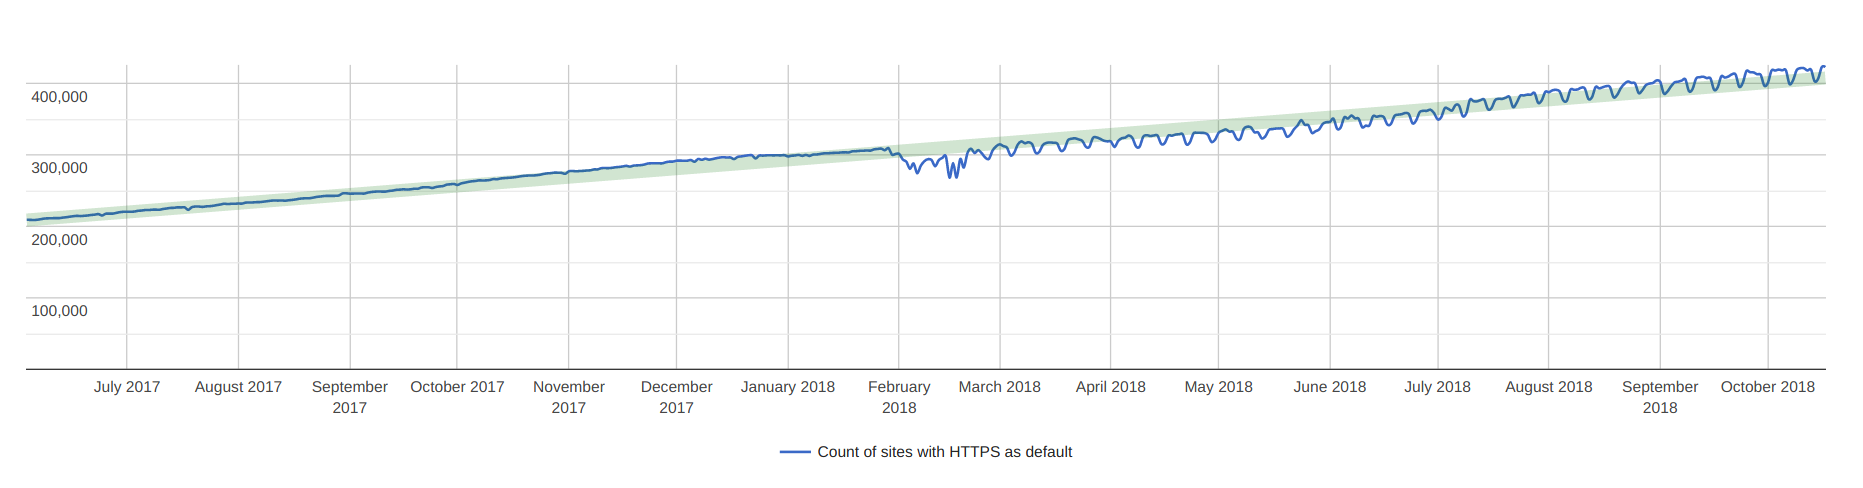
\includegraphics[width=0.9\textwidth]{Figures/httpsRise.png}
  \caption[A graph of HTTPS usage increase]{A graph of HTTPS usage increase\cite{https}}
  \label{fig:httpsRise}
\end{figure}

HTTP is not secure because information transmitted is in plaintext by default and extra steps are needed to encrypt the data. Because the author of the server can choose how the data is encrypted, it can lead to the theft of data as the implementation may not be correct or a weak algorithm is used.
On the other hand if a website uses HTTPS which is a common defined standard there will be minimal data theft see figure \ref{fig:https1}. HTTPS uses SSL or TLS which are protocols that use asymmetric keys (will be discussed later). SSL is generally used more often as it requires the server to acquire an SSL certificate from a trusted third party.

\begin{figure}[ht]
  \centering
      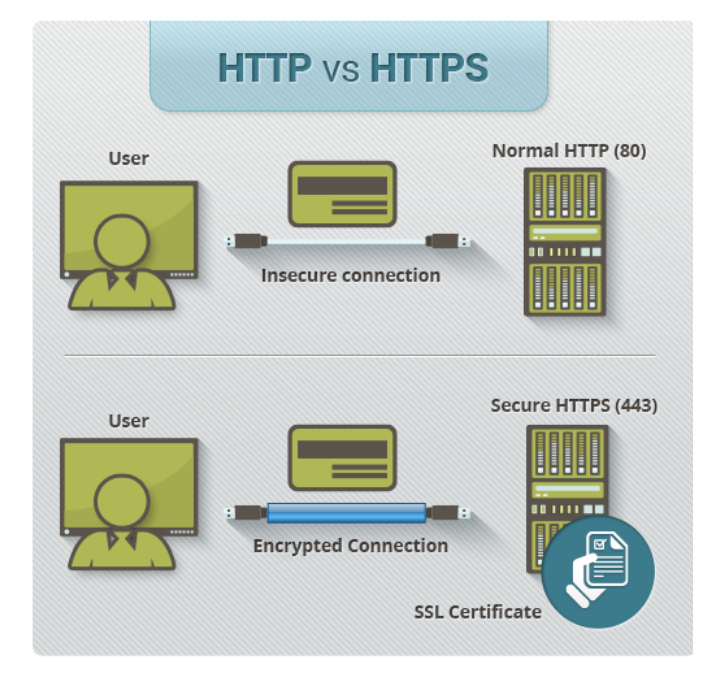
\includegraphics[width=0.6\textwidth]{Figures/httpsVsHttp.png}
  \caption[HTTP vs HTTPS]{HTTP vs HTTPS\cite{https1}}
  \label{fig:https1}
\end{figure}



Traditionally there are two encryption types.
\begin{enumerate}
    \item Symmetric
    \item Asymmetric
\end{enumerate}

Symmetric encryption uses the same key to encrypt and decrypt information. This type of encryption is usually used to encrypt information provided by a human generated key. It is not safe to send this key over a network as it can be stolen or the destination being sent to can be spoofed. There are multiple implementations of symmetric ciphers, the most common being AES, Twofish and Serpent. To increase your security at the cost of encryption and decryption time you can chain multiple ciphers together AES(Twofish(Key)).

Asymmetric or commonly known as public key encryption methods are commonly used for sharing data between between computers on different networks. This is because a set of keys are generated one being private and the other public. The private key is never shared and remains on the host that generated it. The public key on the other hand can be shared with the party you want to communicate securely with. The public key is used to encrypt the data that is about to be sent back. This data can only be decrypted using the private key. Therefore you can share your public key with anyone and they wont be able to decrypt messages sent from another host who used the same public key. The most common algorithm is RSA. Certain protocols also use public key algorithms like SSH for secure remote connections to foreign hosts. And GPG for verification of packages on Linux systems and an alternative over https for Github.

Protocols like SSH create a set of keys during the start of the session and those keys remain constant therefore if the private key was leaked the whole conversation could be decrypted if the packets have been captured and stored.  

Encryption in its general form is simply a mathematical algorithm that takes plaintext and combines it with some sort of key over a number of iterations eventually producing the ciphertext. This might entice some people to try and break those ciphers and recover the original plain text. Quite a number of attacks do exist.
Private keys are sometimes stored on the disk or in temporary files that are saved by programs during their execution, until reboot or they are cleared after a number of days. The attacker may be able to access the server physically or remotely using an unrelated exploit and copy the key.

Social engineering is an attack where a human pretends to be of an authority figure and convinces an unaware human to give up the key. This can be done by an attacker pretending to be an executive engineer in a company and convince the victim indirectly or directly to give up the keys by running obfuscated commands in the terminal which then send over the key to the attackers server.

If the key used is created by a human and not some sort of machine generator there are a few number attacks that can be performed that would not be feasible or possible if the key was generated or quite long. These attacks include brute force which creates keys in usually ascending order or based on some algorithm to increase the chance of success. Brute force will eventually try every key possible however even a small sized key of 12 characters containing numbers, symbols, upper and lover case numbers it would take around 200 years \cite{brute}. 
Dictionary attacks can be used if the key is part of a large dictionary of human created passwords. 

Attacks on proper keys that are generated by machines are more sophisticated and rely on cracking the algorithm or device used for encryption more so then the key.
Linear cryptanalysis \cite{cipher-attacks} is a plaintext attack which means that the attack can use any plain text they want and receive the ciphertext for it after putting it through a system. This attack uses linear approximations to describe the behaviour of the block cipher. After large number of pairs of plaintext and cipher text there is a possibility to learn something about the key.

Algebraic attacks \cite{cipher-attacks} can be used if the ciphers exhibit a high probability of a mathematical structure. 

Reverse Engineering \cite{cipher-attacks} can be used to either examine the source code of the algorithm or disassemble the binary which uses the algorithm to look as the assembly code of the algorithm.
Machine key generators usually use some form of a random number generator which are algorithms that usually take in a seed hopefully something that isn't the current time but that has been known to be used and return a key. Attacks can be made on this number generator if the seed is something predictable or the generator generates predictable numbers. 

If the device on which the algorithm is performing on is an embedded device you can perform side channel attacks \cite{cipher-attacks} where you measure the spikes and frequency of the power consumption when the encryption is taking place. 

%
%
% End of encription 
%
%

Machine learning is a category of algorithms that allow systems to automatically learn and improve from experience without being explicitly programmed \cite{machineLearning}. Basically this means that the algorithm can update when input is received this in turn updates the the output even if the same inputs are used later on.
Typically machine learning software processes large amounts of data and looks for patterns constantly updating either variables or adding logic branches. Recommendation engines use machine learning to personalise the logged in users feed. So if user one looked at product X and user 2 bought product X and also bought product Y then user one will most likely see product Y as a recommendation. There are three types of recommendation systems. Collaborative Filtering \cite{recommendation} where similarities between customers is taken into account.
Content Based Filtering \cite{recommendation} is when the liked and purchased items are taken into account. See figure \ref{fig:recommendation} for illustration.
Finally there is Hybrid Recommendation Systems which is a mix between the previous two and is typically the one used in industry.

\begin{figure}[ht]
  \centering
      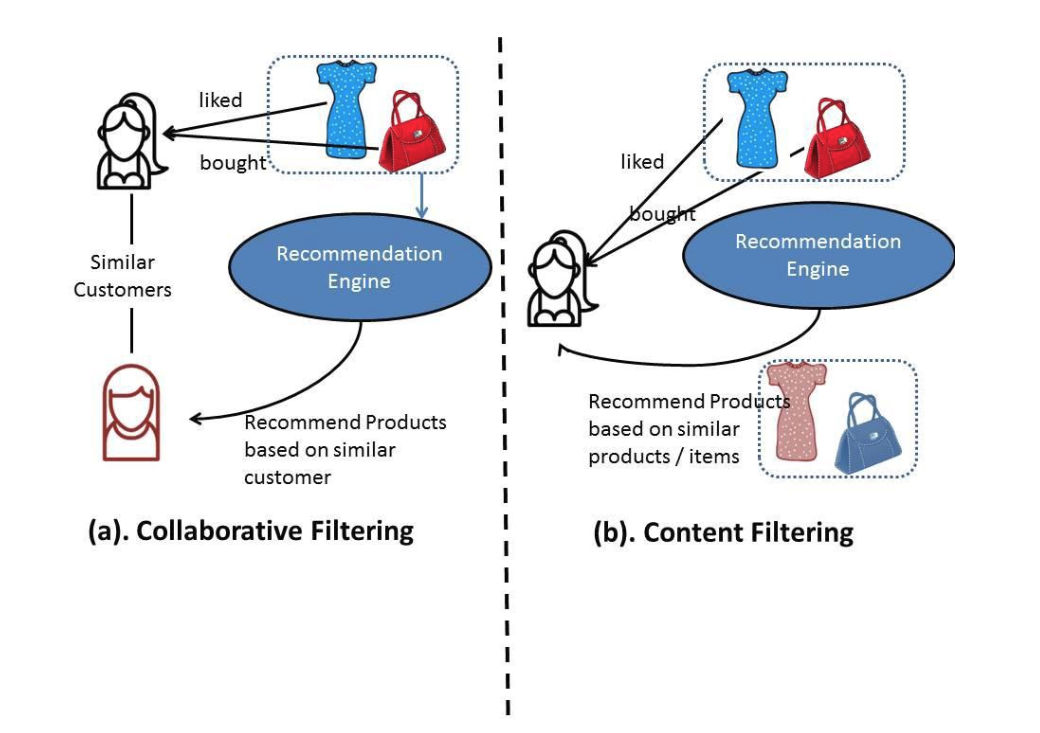
\includegraphics[width=0.9\textwidth]{Figures/recommendationEngine.png}
  \caption[An example of recommendation engine]{An example of recommendation engine\cite{recommendation}}
  \label{fig:recommendation}
\end{figure}

The most common machine learning algorithms are often classified as supervised learning and unsupervised learning.
Supervised learning \cite{supervised} relies on a set of training data which is constructed of various inputs and and correct outputs corresponding to those inputs usually labels. The training data is usually left unchanged and when the test data or data taken from the current user is used as input the algorithm attempts to correctly classify the data based on the training data. The disadvantage of supervised learning is if the incoming data is radically different from the test data the probability of classifying the data into the correct label will be similar and sometimes even lower than classifying into the incorrect label. However because the training data exists it can be quite quicker to setup a supervised learning system then an unsupervised.

Unsupervised learning \cite{unsupervised} uses data that is neither classified or labelled. This allows the algorithm to draw its own conclusions about the data as well as discover hidden structures. If some of the data is similar in any way to another piece of data the algorithm tends to group those pieces of data together. Unsupervised learning is generally more complex and can be more accurate since the algorithm might find subtle discrepancies that might be impossible to notice for a human. This however can lead to unpredictable behaviour where there is expected to be two classifications but instead the data is classified into a lot more than two classifications. Unsupervised learning algorithms typically require more training data than supervised in order to detect similarities and come up with labels.

There are also algorithms that use techniques found in both supervised and unsupervised machine learning these are called Semi-supervised \cite{machineLearning0} machine learning these use a much larger amount of unlabelled training data than labelled. These types of algorithms usually tend to be more accurate than supervised and unsupervised alone.

Another interesting suite of machine learning algorithms is classified into Reinforcement Learning \cite{reinforcementLearning}. These algorithms interact with the environment and received rewards or penalties based on the actions carried out within the environment. If the action carried out receives a reward it is likely that the same action will be repeated again. 

%
%
% End of machine learning
%
%

Achieving synchronisation \cite{sync} is an important part of this project. 
Synchronisation is the process of making two or more data storage devices or programs (in the same or different computers) having exactly the same information at a given time.
Synchronisation is common in multi-threaded software where any number of threads can manipulate the same set of data or even wait for a certain thread to finish execution. For example you wouldn't want your parent thread to finish before the child threads as this can lead to data loss and resources being hogged by a zombie thread. Pthread \cite{pthread} is a great API that can be used for handling threads and shared data between those threads. 
Data Synchronisation \cite{datasync} is an on going process of having the same data present on selected servers. Large databases that operate on multiple servers usually use data versioning to keep check on the latest data. MongoDB is one such database \cite{mongo} this is the reason for a delay when you upload a YouTube video (YouTube doesn't use MongoDB this is just an example) it might not be instantly available for other users to watch as it needs to propagate through a number of servers hosting the databases.
Popular websites use data synchronisation for mirroring websites. This allows users to be distributed among relatively identical servers in order to avoid bandwidth bottlenecks as well as increasing availability just in case one server dies users will be redirected to a different mirror seamlessly without interruptions. 
File synchronisation is the method of choice for home backups this is preferable over the traditional backup methods where data is simply dumped onto another hard drive. This process prevents copying identical files which leads to faster transfers and a less chance of errors occurring. My personal favourite file synchronisation tool is Unison \cite{unison}. It is also possible to synchronise folders over the network between two home computes, Unison does this through SSH.
Blockchain \cite{blockChain} the method used for secure crypto ledgers which also relies on synchronisation between peers. Synchronisation for the ethereum crypto currency blockchain can be expressed as follows. "Synchronisation proceeds from head to known block by requesting and fetching block hashes iteratively from young to old (head to root). Based on block hashes, blocks can be requested. Based on the parenthash of a block, independent sections can be linked and a chain established. By checking if a block is found in the block chain the root of the blockpool can be established and the chain can be inserted in the blockchain."
%#######################################################
%                                                   
% check if its ok to just dump stuff from the web.
%
%#######################################################

%
%
% End of sync
%
%






%
%
% Stick these somehwere maybe 
%
%
Machine learning has been known to be used for secure communications although it is not clear if it is used in servers with valuable data. Google's AI successfully created secure algorithms \cite{GoogleAi1} that use inhuman cryptographic schemes making them harder to crack. This technique is called GAN Cryptography \cite{GoogleAi2} for which a research paper can be found.

Currently dynamic encryption is exercised in voip phone calls by a company known as Dencrypt \cite{dencrypt} according to the explanation of their proprietary algorithm they use a wrapper on top of AES-256 which is a chosen algorithm that is discarded when the data transfer is finished.


This project will be compatible with NodeJs because it is one of the fastest growing server platform \cite{NodeJs} that can be easily set up and supports a large amount of modules.

%
%
% Stick these somehwere maybe ^^^^^^^^^^^^^^^^^^^^^^^^^^^^^^^^^
%
%

%
%
% Notes Start
%
%
Position your topic within Computer Science. This activity will aid you in your literature review also. We zoom out to see three levels:

% notice the enumerate structure to create itemized lists
\begin{enumerate}
    \item What is the core topic your project is about? e.g., Mobile app for online voting.
    \item What core area(s) does the project fall under? e.g., Mobile applications, Social Networking, Service Providers. 
    \item What main area(s) of Computer Science does the project fall under? e.g. Software Development, Cloud Computing.
\end{enumerate}

The ACM Computing Classification System (http://www.acm.org/about/class) will aid you in this, use the 2012 categories. Make sure to use figures and illustrations were appropriate. LaTeX will take care of the formatting of these. Do not try to get fancy here, you should concentrate on the content and not the formatting, this is why we are specifying LaTeX.

% Again take note of the structure, simply copy and paste this for future single figures
\begin{figure}[ht]
  \centering
      
\includegraphics[width=0.7\textwidth]{successkid.jpg}
  \caption[A picture of the success kid!]{A picture of the success kid!\cite{Reference1}}
  \label{fig:successkid}
\end{figure}

You can specify the width and label for a figure which allows you to reference the figure and you can attribute a source in the figure caption as is done for figure \ref{fig:successkid}. Make sure you reference all external figures (i.e. figures you did not create yourself). Also use references for all figures e.g. use "... in figure \ref{fig:successkid} ..." NOT "... in the figure above ...".

%\section{Project Scope}
%Project specifics: Background minimum knowledge.

%Imagine you wanted to explain the specifics of your project to a person that knows nothing of Computer Science. You cannot talk about everything (as the idea is not to write a 500+ page report). Remember the reader at this stage can only be assumed to know what you have covered, so identify what are the minimum concepts belonging to the main areas (listed as 3 in the section before) and the core areas (listed as 2 in the section before) that you would need to explain so that the reader is able to understand the specifics of your project and indeed the following section. For example the minimum amount of knowledge about software development, cloud computing, mobile applications, social networking and service providers that are required so as to understand the specifics of a project about a mobile app for an on-line voting system. Here we are making the same trip we did before, but now in the opposite direction. Start zooming in from 3, then to 2 and finally to reach your project 1. Once the reader is finished this section they should be able to understand the proceeding sections (and have context for it within the project).
%
%
% Notes End
%
%

%
%
% Notes 2.2 Start
%
%
\section{A Review of -INSERT THEMATIC AREA-}
The focus of this section is at the heart of the project research phase. You must identify the main sources of information you should be aware of within your chosen area and pay regular attention to so as to strengthen your knowledge in the core topic you are working at. So here you should develop an knowledge of not only your core topic but also about the area of computer science the topic falls under. More specifically you should research the following:
\begin{itemize}
    \item The top 5 International Conferences and Journals most related to your topic. This is crucial, as it represents the main source for keeping you aware of what the state-of-the-art in your topic is.
    \begin{itemize}
        \item In particular it will make you aware of what other projects related to yours have been already done (so that you can compare/position your project w.r.t. these).
        \item What new techniques are being developed, so that you can apply them in your work. e.g. new frameworks for data visualization
    \end{itemize}
    \item The top 3 most recent books/texts related to your topic. There are many free resources from which you may download a relevant text on the topic of your project. Try to either download or borrow 3 recent (no older than 10 years) texts relating to the topic your project is on which you will use throughout the project as reference material and to aid in tackling a number of the technical problems you may encounter. Any PhD/MSc thesis that have published in the last 5 years relating to the topic are also invaluable resources as they will contain a state of the art and references in your project topic. Approach these only after reading/viewing the wikis/Youtube videos you find as a certain level of knowledge will be assumed about the topic.
    \item The top 5 companies/organizations potentially interested in the product you are developing. Finally, this is also crucial, as it forces you extend to purely programmer view of the project to a wider view considering the market, potential stakeholders and niches where your product can become useful. Moreover, Computer Science is a huge topic with loads of different works and roles. If you pick a project in the area you feel passionate about, and you identify what the market in this area is about, then you can drive your future professional career (from the very beginning) towards the path that makes you happier. I know that this does sound as a very technical reason, but I suppose we all agree is probably the most important of all reasons for choosing a particular project focus. 
    \item The top 5 wiki/forums/blogs/Youtube channels most related to your topic. This is crucial to you as well, as it represents a more accessible, personal and less informal way of communication with people working/interested on the same topic as you are. This communication is extremely helpful for improving your skills, solving potential doubts and increase the interest/relevance of the topic/area itself.
\end{itemize}

You should begin your journey of discovery in reverse order to the listing above (which is given in order of academic importance/significance). So when you are researching your topic first look up some TedX talks or youtube tutorials, then research what companies are doing in the area, then get a handful of very good texts on the core topics of your area (anything older than 5 years usually is not helpful here) and finally start reading conference or journal papers (again newer is better here). In particular during this section you may need to use tables to list resources. These are also automatically formatted in latex thus allowing you to concentrate on content. for example table \ref{tab:Mylar}.

\begin{table}[ht]
	\centering
		\begin{tabular}{ c  c  }
		\hline
		\hline
		Parameter & PET \\
		\hline
		Youngs Modulus & 2800-3100MPa \\
		Tensile Strength & 55-75MPa \\
		Glass Temperature & 75$^\circ$C \\
		Density & 1400kg/m$^3$ \\
		Thermal Conductivity & 0.15-0.24Wm$^{-1}$K$^{-1}$ \\
		Linear Expansion Coefficient & $7\times10^-5$ \\
		Relative Dielectric Constant @ 1MHz & 3\\
		Dielectric Breakdown Strength & 17kVmm$^{-1}$\\
		\end{tabular}
	\caption{PET Physical Properties}
	\label{tab:Mylar}
\end{table}

What has been done before in your community w.r.t. your topic? Once you have gotten an understanding of the topic and technologies and have identified the top 5 formal conferences/journals, wiki/forums/blogs/Youtube channels and companies/organizations the next step is to research in depth on them! And here in depth means in depth. Make sure you cite\cite{Reference1} a number of papers \cite{Reference3}, luckily Latex will take care of the ordering of the citations \cite{Reference2} for you.

The aim here is that you find the trends in your topic (3), and more in general in the area in which your topic resides (2) your project falls under and from these trends you develop your initial project question further and begin to get insights into how others have solved/approached similar problems. Think of this section as colouring in your initial idea. Before you approach this section you should read at least 4/5 good literature reviews (a selection of last years projects will be posted on blackboard to aid you but you should find other sources also).

In particular in this section, you must find and analyse at least 5 (ideally around 10) works belonging to, or at least related to, your work. You must describe these works and position your project w.r.t. them (i.e., clearly identify the similarities and differences between your project and each of these works). Also remember if you find that you are detailing topics that you have not introduced already here you need to add something to the earlier Scope section.
%
%
% Notes 2.2 End
%
%

%
%
% Research papers
%
%
To achieve my goal of dynamically encrypting messages between both parties, each party must know the encryption key without explicitly sending that key to each other. For this to have a dynamic effect multiple processes will in this case synchronise which each other and a separate process will take care of swapping keys.

The research papers that will be cited synchronise once therefore I will just have to take what I learned and apply it to multiple instances.

Two identical neural networks that originally have a random generated state. This state is different between the two networks and to achieve synchronisation this state must be the same, this is because when the state is the same it will be essentially the key used to encrypt messages. And all this will be achieved without ever sending the key over the network even in an encrypted form as in public private encryption techniques. 

A tree parity machine is a common method used across all papers in order to achieve this goal figure \ref{fig:treeParityMachine} visualises such a machine.

\begin{figure}[ht]
  \centering
      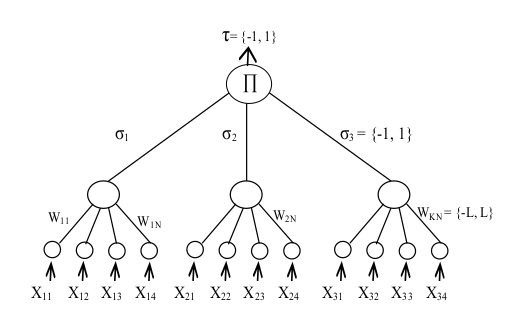
\includegraphics[width=0.7\textwidth]{treeParityMachine.png}
  \caption[Tree parity machine]{Tree parity machine with L=[-4,4], K=3 and N=4\cite{Private_Inputs_to_Tree_Parity_Machine}}
  \label{fig:treeParityMachine}
\end{figure}

According to \cite{Genetic_Key_Guided_Neural_Deep_Learning_based_Encryption} both parties should have the same layout of the tree parity machine where N is the number of neutrons used as input for each hidden neutron. The input neutrons have the X and are at the bottom of the diagram, in this case there are four input neutrons for each hidden neutron. The hidden neutrons are referenced as K, these are the neutrons in the middle with the W in the diagram. These are the weights which are updated if the output of both of the tree parity machines are the same. These weights in the end will be the key used for symmetric encryption between the two parties. T will be the output value which will be compared to the other tree parity machine. 

There is a low number of machine learning algorithms that can be used to synchronise and the paper \cite{Genetic_Key_Guided_Neural_Deep_Learning_based_Encryption} as well as the majority of papers use the hebbian-learning rule figure \ref{fig:hebianFormula}

\begin{figure}[ht]
  \centering
      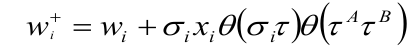
\includegraphics[width=0.7\textwidth]{hebbian_learning.png}
  \caption[Hebbian learning rule]{Hebbian learning rule\cite{Genetic_Key_Guided_Neural_Deep_Learning_based_Encryption}}
  \label{fig:hebianFormula}
\end{figure}

The other two learning rules that can easily be substituted according to this paper \cite{DESIGN_OF_AN_EFFICIENT_NEURAL_KEY_GENERATION} are as follows anti-hebbian learning rule figure \ref{fig:antihebbianlearning} and random-walk rule figure \ref{fig:randomwalklearning}.

\begin{figure}[ht]
  \centering
      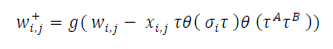
\includegraphics[width=0.7\textwidth]{anti-hebbian.png}
  \caption[Anti-Hebbian learning rule formula]{Anti-Hebbian learning rule formula\cite{DESIGN_OF_AN_EFFICIENT_NEURAL_KEY_GENERATION}}
  \label{fig:antihebbianlearning}
\end{figure}

\begin{figure}[ht]
  \centering
      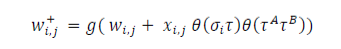
\includegraphics[width=0.7\textwidth]{random-walk.png}
  \caption[Random-Walk learning rule formula]{Random-Walk learning rule formula\cite{DESIGN_OF_AN_EFFICIENT_NEURAL_KEY_GENERATION}}
  \label{fig:randomwalklearning}
\end{figure}

There are a number of steps involved in synchronising the tree parity machines.
Step 1. The weights at the beginning should be randomly initialised using local randomisation techniques because there is a chance that downloading data from random APIs can be spoofed which will result in the attacker easily synchronising with your tree parity machine. 

Step 2. Generate random input which will be used by both of the tree parity machines. This input can be generated by a third party server or one of the two parties.

Step 3. Calculate the value of the weights based on the random input using the formula in figure \ref{fig:hiddenNeutronFormula}

\begin{figure}[ht]
  \centering
      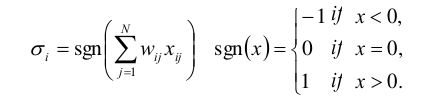
\includegraphics[width=0.7\textwidth]{hidden_neutron_folmula.png}
  \caption[Hidden neutron formula]{Hidden neutron formula\cite{Genetic_Key_Guided_Neural_Deep_Learning_based_Encryption}}
  \label{fig:hiddenNeutronFormula}
\end{figure}

Step 4. Calculate the output neutron based on the weights using the formula in figure \ref{fig:outputNeutronFormula}

\begin{figure}[ht]
  \centering
      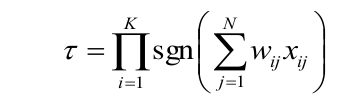
\includegraphics[width=0.7\textwidth]{outputNeutronFormula.png}
  \caption[Output Neutron Formula]{Output Neutron Formula\cite{Genetic_Key_Guided_Neural_Deep_Learning_based_Encryption}}
  \label{fig:outputNeutronFormula}
\end{figure}

Step 5. exchange the output between both of the tree parity machines through a network and if the outputs are not the same repeat again from step 2. And if the outputs are the same apply the hebbian learning rule to the weights and update them accordingly. Repeat step 3 to step 5 until both of the tree parity machines have the same weights.

This technique can be considered too simplistic and the attacker has a greater probability in synchronising with the two parties. I will cover attacks related to tree parity machines further in the section.

To increase the speed of synchronisation and lower the chance of the attacker being able to synchronise with the parties. A technique called queries is used \cite{Private_Inputs_to_Tree_Parity_Machine}.
This technique replaces step 2 from before where the input would be randomly generated by a third party or one of the party. A query consists of a generated vector based on a field of the weights. These queries are then sent from each party to the other interchangeably. 
To calculate the new local field value the following formula can be used figure \ref{fig:LocalFieldFormula}
\begin{figure}[ht]
  \centering
      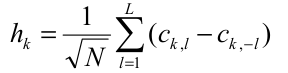
\includegraphics[width=0.7\textwidth]{syncQueriesLocalField.png}
  \caption[Local Field Formula]{Local Field Formula\cite{Private_Inputs_to_Tree_Parity_Machine}}
  \label{fig:LocalFieldFormula}
\end{figure}

It is possible to use a different algorithm where the output \[\sigma_k \] is chosen random for the hidden unit.
It is possible to use the following formula to calculate the local field value. \[ h_k = \sigma_k H \]

To calculate the list of c values that will be used to affect the generation of input values it is possible to use the following two formulas. 
\begin{figure}[ht]
  \centering
      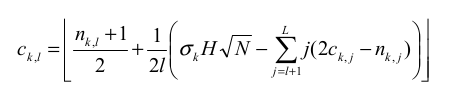
\includegraphics[width=0.7\textwidth]{cformulaa.png}
  \caption[C Formula one]{C Formula one\cite{Private_Inputs_to_Tree_Parity_Machine}}
  \label{fig:LocalFieldFormula}
\end{figure}
\begin{figure}[ht]
  \centering
      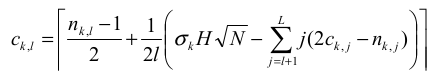
\includegraphics[width=0.7\textwidth]{cformulab.png}
  \caption[C Formula two]{C Formula two\cite{Private_Inputs_to_Tree_Parity_Machine}}
  \label{fig:LocalFieldFormula}
\end{figure}

Where one formula is chosen randomly in each calculation. The probability of one formula being chosen is 50 percent.
Th inputs are then generated and if the inputs are associated with zero weights then the inputs are randomly generated since they do not influence the local field value. 
The input is then divided into L groups and are selected randomly and assigned to \[x_k,_j = sgn(W_k_j) \]
% this double subscript error is fine displays as it should
Finally the remaining input values are set to  \[x_k,_j = -sgn(W_k,_j) \]
To achieve secure key exchange with queries the parties should choose the parameter H so that they can synchronise quickly while the attacker would not be able to do so in time.
Despite the queries being based on the weights an attacker cannot predict the query generated by either party since the weights are never shared. Therefore an attacker can collect the queries but won't be able to establish a mathematical connection between them.
After the synchronisation is complete the weights can be used as a seed for a random generator. As the attacker doesn't know this seed the output of this generator won't be predicted.

There are a number of different attacks that can be carried out on the tree parity machines. These attacks are  more successful if using the basic synchronisation method without the use of queries. This is because up to this date there is no documented or rumoured methods of being able to synchronise with parties who are using queries.

The most basic and useless attack would be a brute force.
This involves trying every possible values for the weights. If using a tree parity machine consisting of 3 hidden neurons, 300 input neurons and 3 weights will result \cite{Private_Inputs_to_Tree_Parity_Machine} in \[3*10^2^5^3\] possible values for the weights making this attack quite impossible using modern computing power. 

The attacker can attempt to learn the weights by using their own tree parity machine with the same number of hidden neutrons and inputs \cite{Private_Inputs_to_Tree_Parity_Machine}. This is essentially identical to the parties tree parity machines but with different initial weights and the attacker synchronises indirectly.
There are three possible situations that can occur with this attack. In these situations A and B will be the two parties trying to synchronise and E is the attacker.
situation 1. Output of A doesn't match output of B and therefore none of the parties including the attacker update their weights.
situation 2. Output of A matches output of B and output of E is also the same. This time A, B and E update their weights.
situation 3. Output of A matches output of B but output of E doesn't match. parties A and B update their weights but E cannot do that and therefore it will take E more time to synchronise to A than it would for B to synchronise with A. Because the learning is ceased after A and B are synchronised E will be left in the dark and not synchronised state. You can further decrease the success rate of this attack by increasing the synaptic depth of the neural network \cite{Private_Inputs_to_Tree_Parity_Machine}. Increasing this will have a performance impact on the parties polynomially however the chance of successful attack decreases exponentially.

More sophisticated attacks can be found in this research paper \cite{BIG_ResearchPaper} such as the genetic attack.
This uses a form of genetic algorithm the key to a successful attack using this method revolves around E being able to determine the fitness of her neural networks.
The attacker spawns a number of tree parity machines which attempt to synchronise with A. After a set time period a selection is made where the most successful synchronised tree parity machines are used to generate the next population. This selection works best if there are certain observable differences between attractive and repulsive effects. 
This attack can be quite successful if the synaptic depth of the neural network is not too large. This can be expressed with the following formula in figure \ref{fig:geneticESuccess} where the probability of E being successful decreases exponentially with the synaptic depth L.
\begin{figure}[ht]
  \centering
      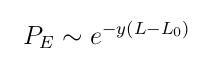
\includegraphics[width=0.3\textwidth]{geneticFormula0.png}
  \caption[probability of E being successful]{probability of E being successful\cite{BIG_ResearchPaper}}
  \label{fig:geneticESuccess}
\end{figure}

In order for this attack to be likely successful the number of tree parity machines the attacker will use will need to be exponentially increased with the increase of the synaptic depth see figure \ref{fig:geneticEMachine}.
\begin{figure}[ht]
  \centering
      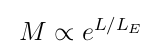
\includegraphics[width=0.3\textwidth]{geneticFormula1.png}
  \caption[Tree Parity Machines needed for synaptic depth]{Tree Parity Machines needed for synaptic depth\cite{BIG_ResearchPaper}}
  \label{fig:geneticEMachine}
\end{figure}
 % Background Theory 

\chapter{Problem - rename to project title}
\label{chap:problem}
\lhead{\emph{Problem Statement}}
The key question to be addressed in this chapter is: "What do I want to achieve".

This chapter should comprise around 1500 words and describe the problem you are trying to solve. Try to be as specific here as you can, this will help you to anticipate possible risks such as lack of support from APIs.

\section{Problem Definition}
Describe the problem you are trying to solve in this project. There will sometimes be a need at some point during the report to display an equation that may be core to your project. For example if the project is on gait detection what equation are you using to determine gait? If the project is on localization what is the method/formula? The formatting of these is reliably done in Latex also as we can see in equation \ref{eq:Legrange}.

\begin{equation}
\frac{d}{dt}(\frac{\partial L}{\partial \dot{c_i}})-\frac{\partial L}{\partial c_i}+\frac{\partial P}{\partial \dot{c_i}} = F_i,
\label{eq:Legrange}
\end{equation}


\section{Objectives}
Enumerate the objectives you want to achieve in your project. Again as this is an early stage these will tend to change but there should be a rational explanation for this change. Always document your work, keep a lab book during the term that you only use for FYP!

\section{Functional Requirements}
Enumerate the functional requirements you want your project to have. 

Please, do not include the use cases here. If you want to create a one-to-one mapping between functional requirements and use cases (which does not necessarily need to be the case, indeed most likely this will not be the case) do it elsewhere. Here should purely describe what do you want to do. In no case should you use this section to provide a description of how to implement them, that is for later. For people doing projects that are not heavy implementation projects (e.g. deploying an architecture or testing a novel tool in specific conditions) this structure can still be used as it will force you to think about what you plan to achieve and what possible metrics you may need to measure success.

Let me explain this with more detail. A common mistake is that people confuse the problem description with the solution approach. This is a common mistake by confusing the \emph{what} with the \emph{how}. Here we are purely focused on the what: What is this project about? What are the objectives? What are the functional and non-functional requirements? 

How are we going to do all these things? Well, this is a question for next chapter. Provided a problem, an objective or a functional requirement, obviously there will usually be many ways of doing it, thus there will be many \emph{hows}, but the definition, the \emph{what} we want to achieve will be unique.

One other display structure you may wish to use at some stage during the report is a figure array. This can also be easily done with Latex and is shown in figure \ref{fig:twosuccesskid}

\begin{figure}
\centering     %%% not \center
\subfigure[Figure A]{\label{fig:a}
\includegraphics[width=0.48\textwidth]{successkid.jpg}}
\subfigure[Figure B]{\label{fig:b}
\includegraphics[width=0.48\textwidth]{successkid.jpg}}
\caption{Two Success kids}
\label{fig:twosuccesskid}
\end{figure}

\section{Non-Functional Requirements}
Enumerate the non-functional requirements you want to achieve in your project (i.e. broadly speaking how your system will operate).

 % Problem

\chapter{Implementation Approach}
\label{chap:implementation}
\lhead{\emph{Implementation Approach}}
The key question to be addressed in this chapter is: "How do I plan to achieve what I have outlined in the previous chapter".

This chapter should comprise around 5000 words and specify your planned implementation approach. Again all sections below are suggestions and will vary significantly from project to project, the key element to be addressed is the core question of the chapter.

\section{Architecture} \label{sec:Arch}
Describe the architecture of the solution that you have in mind, including:
\begin{itemize}
    \item Technologies involved (e.g., frameworks, programming language). 
    \item The hardware needed to develop the project (and to support at deployment stage)
\end{itemize}

Provide a high level view of the system you have in mind, including any package of classes, what is it responsible for and what other packages it communicates to. Provide a high level view of the database (or structure) needed to support the project, including what each table/document is responsible for and the hierarchy among them. You need to be as specific here as you can, why? Because this will aid you in identifying parts of the project you are vague on, this may be fine for some components but cause problems in term 2 for others. If you have hardware element in your project this is also where you provide a high level view of how these elements integrate into the project. So for a project that is cyber-physical you will have both a hardware and software architectural diagram. N.B. This is NOT a full system design but a high level overview of what you can credibly develop. This architecture should be informed by prototyping activity. 

Some of the implementation focused projects may describe how do you envision tackling the functional requirements of your project via a set of use-cases. DFDs are also helpful here to understand elements of your project that may cause problems. You should describe the role of the different parts of the architecture of the solution, and the interaction among them.

\section{Risk Assessment}
Identify any potential risk precluding you from successfully complete your project. This section is really important and often neglected by students resulting in fatal risks occurring in some projects. Make sure to give this section the time it requires. Classify the risk according to their importance, possibility of arising and enumerate the decisions you can make to anticipate them or mitigate them (in case they finally arise). Table \ref{tab:ProjRisks} may help with this classification. This section should include your mitigation approach for any critical risks.

\begin{table}[h]
\centering
\scriptsize
\caption{Initial risk matrix}
\begin{tabular}{|p{2cm}|p{2cm}|p{2cm}| p{2cm} |p{2cm}| p{2cm}|}
\hline \bf Frequency/ Consequence & \bf 1-Rare & \bf 2-Remote & \bf 3-Occasional & \bf 4-Probable & \bf 5-Frequent\\ [10pt]

\hline \bf 4-Fatal & \cellcolor{yellow!50} & \cellcolor{red!50} & \cellcolor{red!50} & \cellcolor{red!50} &\cellcolor{red!50} \\ [10pt]

\hline \bf 3-Critical &\cellcolor{green!50} & \cellcolor{yellow!50} & \cellcolor{yellow!50} & \cellcolor{red!50} &\cellcolor{red!50} \\ [10pt]

\hline \bf 2-Major & \cellcolor{green!50} & \cellcolor{green!50} & \cellcolor{yellow!50} &\cellcolor{yellow!50} &\cellcolor{red!50} \\ [10pt]

\hline \bf 1-Minor & \cellcolor{green!50} & \cellcolor{green!50} & \cellcolor{green!50} &\cellcolor{yellow!50} &\cellcolor{yellow!50} \\ [10pt]
\hline
\end{tabular} \\
\label{tab:ProjRisks}
\end{table}

\section{Methodology}
Describe your personal approach on how to tackle the different parts of this project, including:
\begin{itemize}
    \item How to tackle the needed research to fulfill the background chapter. 
    \item How to set up your Computer Science skills to the project needs (e.g., describe your plan to learn any new technology involved on the project that you are not familiar with). 
    \item What core project managing approach will you follow (e.g., Waterfall, Scrum, etc).
\end{itemize}

\section{Implementation Plan Schedule}
Come up with a schedule for the remaining time (including second semester), so as to describe how do you envision to achieve the implementation of your project by the end of semester 2. This plan SHOULD be ambitious but MUST be realistic and SHOULD be informed by early prototyping and MUST be discussed with your term 1 supervisor.

\section{Evaluation}
Come up with an evaluation plan that allows you to measure how much have you actually achieved the goals of your project. This again is a section that is often neglected where students loose marks. How do you plan to measure the output of your project? A binary it works/does not work is insufficient. You need to be able to quantify the success against both the functional requirements and the initial idea. These are not the same as you may meet all function requirements outlined but not solve the overall problem because you have failed to revisit these and update them with new information which you learn as you are developing the project.

\section{Prototype}
Although you do not have a fully functional project yet, you should show wireframes, snapshots or representation on how do you envision your project to look once the implementation phase has been completed. The nature of this section will vary significantly from project to project and can include anything from code snippets to snapshots of service deployments. Any prototyping you have done during the term should be summarized here that has not been captured in earlier sections. For example if you are planning to host your project using AWS in an EC2 instance you should have at least created a "hello world" setup to determine the basics, this probably should have been discussed in section \ref{sec:Arch}. % Solution Approach

\ifimp
\chapter{Implementation}
\label{chap:imp}
\lhead{\emph{Project Implementation}}
%This chapter should comprise 15 pages and enumerate your experience when doing what you wanted to do the way you wanted to do it.
The implementation of the system has changed drastically since the original plan due to an oversight where it was believed that the Pistache framework could handle the functionality for both the API and the synchronisation between the tree parity machines. The project turned out to be much more involved and difficult than originally expected. This means that the original sprint plan is no longer representative of the actual sprint plan used. This is however to be expected in an agile environment where the following sprint is normally determined after the evaluation of a sprint that was just completed. Despite all of this the system is functional and produces the same outcome as intended.

\section{Difficulties Encountered}
%Enumerate the different difficulties you have found when developing your solution approach. Create three categories of difficulties:
%\begin{itemize}
%    \item \textbf{Easy}: You managed to solve the problem with little difficulty.
%    \item \textbf{Medium}: It was not easy to solve, but you managed to develop a workaround or solution and %still achieve the functionality you originally had in mind.
%    \item \textbf{Hard}: The difficulty was so complicated that you didn’t managed to solve it. As a result, some functional requirement / non-functional requirement or use case from your solution approach was not achieved.
%\end{itemize}

%For each difficulty, classify it into easy, medium or hard. Then, provide the following info:
%\begin{enumerate}
%    \item Description of the difficulty: Brief description of the problem you found.
%    \item How did it affect the original project design?: Indicate how this difficulty affected:
%    \begin{enumerate}
%        \item the architecture of your solution
%        \item if it represented a risk to your project
%        \item if it affected your methodology to develop your project
%        \item if it changed your implementation schedule
%        \item if it changed the evaluation plan
%    \item What did you do to manage the difficulty arisen?: Brief description of your decision to overcome the %difficulty.
%    \end{enumerate}
%\end{enumerate}
The major difficulties I encountered were primarily related to the architecture of the project. The initial class diagrams were way too basic and didn't account for the fact that Pistache would now only be used for the API and nothing else. 

\textbf{Easy Difficulty}
\begin{enumerate}
\item The NodeJs module was replaced with simply a NodeJs App. The NodeJS module is not implemented due to a time constraint and is not necessary to the outcome of the project. The NodeJs module was originally meant to simplify the communication with the API for people who wish to use it. A NodeJS App would need to be implemented regardless in order to use that module and demonstrate the usability of the API. 
The API doesn't have many routes to use therefore it would not be difficult to use the API with any NodeJs App as interacting with the API is simply done with POST requests. The final NodeJs App that is in the same GitHub repository, consumes the API perfectly as well as purposely demonstrating some aspects of dynamic cryptography that would normally be hidden. Any user that wishes to use the API can simply copy the functions in the NodeJs App that interact with the API and change them accordingly to send and receive their own data. It is recommended for users to copy said functions as there are specific steps that need to take place to register the NodeJS App with the API in particular the synchronisation service. For this reason The NodeJs App uses pure NodeJs libraries like ExpressJs \cite{ExpressJS} which is the most popular routing framework for NodeJs. The NodeJs App has no front end as it would be difficult for users wishing to use the API to adapt the front end too, therefore only a basic HTML template engine is used to deal with the HTML. JavaScript for the front end is purely used for visual purposes and is not required since all of the information sent from the browser to the NodeJs app is done through classic HTML forms. This doesn't have any impact on the architecture as the NodeJS App is not really included in the architecture as it is simply designed to consume the API. This does impact the schedule in a positive way as it is easier and quicker to simply make a NodeJS App than a NodeJs module and a NodeJs App.
\end{enumerate}

\textbf{Medium Difficulty}
\begin{enumerate}
\item The sprints needed to be adjusted to accommodate the new implementation plan. The final sprint plan will be placed here as it briefly reflects the major changes that took place, these changes will be discussed in more detail in the following sections. The Sprint plan follows a two week sprint approach.
\begin{table}[h]
\centering
\caption{New Sprint Plan}
\begin{tabular}{|p{1cm}|p{12cm}|}
\hline Sprint & Tasks \\ [14pt]

\hline 1 & Create a basic API server that can process GET and POST requests. Familiarise self with RapidJSON library \cite{rapidjson} and create functions to parse C++ objects into JSON "strings" and JSON "strings" back into C++ objects. Research peer to peer libraries, no useful ones were found. Decided to make a custom one with the help of the Boost ASIO \cite{boost_asio_home} library. Never used Boost ASIO before therefore a decision was made to follow the developers tutorials on the Boost ASIO website. This was not enough to understand the complicated library therefore other tutorials such as this one \cite{boost_asio_totorial_1} were also followed.  \\ [12pt]

\hline 2 & Further knowledge of Boost ASIO needed to be acquired before it was possible proceed with coding the actual peer to peer network. Thankfully a very informative book called Boost.Asio C++ Network Programming \cite{boost_book} by John Torjo was purchased and ended up being the last resource needed in order to complete the peer to peer network. A basic peer to peer network was written however was unstable at the end of this sprint \\ [12pt]

\hline 3 & Peer to peer network works. Implemented basic synchronisation with real tree parity machines. Implemented command line parsing using Boost Program Options \cite{boost_asio_cmd} to enable different options such as selective outputs and port configurations. Completed synchronisation between tree parity machines fully therefore they produce the same weights successfully. Implemented "logging" to external terminal windows. \\ [12pt]

\hline 4 & Research how to proceed with the API i.e have two separate processes or contain the API and peer to peer network within the same process. Decision was made to contain both in the same process for security reasons. Basic API server was constructed and could be easily spawned along side the peer to peer service.\\ [12pt]

\hline 5 & Implement API functionality for synchronisation. Changes needed to be made to the peer to peer service to accommodate unexpected requirements needed to begin synchronisation when using the API. AES encryption decryption implemented using Crypto++ \cite{cryptopp} library. Encrypted data needed to be encoded using base64 again with the help of Crypto++ library. Implement a NodeJs app to consume and demonstrate various features of the API.\\ [12pt]

\hline 5 & Test the system. Implement options to choose which parts of the system to log since logging everything at once can be difficult to demonstrate different aspects of the system. \\ [12pt]

\hline
\end{tabular} \\
\label{tab:ProjRisks}
\end{table}

\FloatBarrier



\item The API and the synchronisation could not be done using only the Pistache framework as originally believed. This was a fairly significant set back since I have experimented before with Pistache framework and was familiar with how it operated functionality wise. It was only until I attempted to use Pistache for synchronisation I discovered that my original plan will not work since Pistache is a very good REST framework and not much else. To synchronise the tree parity machines a peer to peer network seemed most appropriate in how the synchronisation was envisioned to take place. After searching for easy to use libraries that supported peer to peer networks nothing that matched the requirements was found. This lead to the conclusion that a custom peer to peer network would have to be built from scratch. The attention grew towards Boost Asio as it is the most flexible generic networking library for C++. Unfortunately this library is quite extensive and is not as abstract as some of the previous peer to peer libraries encountered. Since with Boost Asio you will still deal with sockets however this will allow for greater control provided you know how the library works and Boost Asio has excellent asynchronous support which is essential for a responsive server. It took almost two full sprints to learn how the library works which set my initial schedule back as it was planned to spend time to learn the new technologies that would be used however it was not expected to spend so much time learning said new technologies. However some of the lost time was made back since the design of the peer to peer network was simple and efficient which allowed for a large number of synchronisation requests to take place per second resulting in generating a valid key in around one second which satisfies the requirement and no further optimisations needed to take place. This occurrence changed the architecture significantly since originally this wasn't meant to be present. Overall I'm glad that this happened as I had a chance to learn one of C++'s most popular networking library. Another benefit of using Boost Asio for synchronisation over Pistache apart from the fact that its impossible to achieve using Pistache is because the Boost Asio library is a lot lighter the performance increase is rather large. Obviously this would be impossible to test fairly however based on Pistache stress tests it can manage roughly 300 - 400 requests per second. The peer to peer Boost Asio can process around one thousand requests per second as it takes around one thousand requests for the tree parity machines to synchronise and they synchronise generally once per second.

\end{enumerate}

\section{Actual Solution Approach}
In December of last year, when writing the first version of the report, in Chapter 4 you came up with your original solution approach. On it, you presented (i) the architecture of your solution, (ii) your list of use cases, (iii) a risk assessment, (iv) a methodology to develop your solution approach, (v) your implementation schedule, (vi) your evaluation plan and (vii) some prototype of the resulting product. From January to April you have been developing your solution approach. Along the way you have encountered difficulties (the ones listed in Section 5.1) which might have modified your original plan so that you can come up with an actual developed project.

This section is effectively the production of "as built" specification where you compare your original design to the final finished project. Please go section by section (the ones listed from (i) to (vii) in the last paragraph. For each section, enumerate any difference between the original design and the final project, and justify the difficulty forcing you to make such this change. Do not fret if some of these changes are radical, what is important here is that there is a clear rationale for changes made. % Conclusions and Term 2 work
\chapter{Testing and Evaluation}
\label{chap:eval}
\lhead{\emph{Project Testing}}
%The goal of this chapter is an objective evaluation of the final system. The evaluation must be quantitative and not qualitative. You may perform qualitative evaluation but this should not form the basis of the main conclusions you derive from the evaluation. This evaluation, where possible, should be comparative, i.e. you should evaluate your system against a commercially available system and/or system detailed in a research publication. You should demonstrate operational testing of the project using real or contrived data sets to evaluate aspects of the project not encompassed in the software testing (e.g. quantify how well does your project achieved the overall goal). 
%\begin{itemize}
%    \item For software based projects this will include, but should not be limited to, evaluation of non-functional requirements.
%    \item For infrastructural projects this testing should include system/network KPI analysis.
%    \item For analysis based projects (ML, malware or other) this may include model evaluation or YARA rule validation, for example.
%    \item For management projects, where software testing or infrastructure testing may not be in scope, the test process for the system is expected to be more rigorous and well described than a project incorporating significant development work.
%\end{itemize} 
%
%Some suggested sections (the nature of this chapter should be discussed in detail with your term 2 supervisor):
%
%\section{Metrics}
%Identify and describe the metrics you used to evaluate your project. You should have identified some of these in the research phase report but will detail these as you progress through the design.
%
%\section{System Testing}
%Describe the experimental setup for each metric, and how you obtained the measurements. Describe the inputs for each experiment
%
%\section{Results}
%Summarise the output data, and the statistical or other techniques to deduce your results. Summarise your results, including tables or graphs as appropriate with a brief description of each. here possible, compare your results with other products/systems. Identify any possible threats to the validity of your results, and discuss each briefly here (you will discuss in more detail in the next chapter).
%
This chapter will go into more detail into how DynamiCrypt actually works. There will various code snippets present throughout this chapter. After an explanation of how parts of the system work tests will also be carried out. 

\section{The Beginning}
C++ is a compiled language and DynamiCrypt requires quite a few libraries to be present for linking. The command to compile DynamiCrypt is the following.
\begin{lstlisting}
g++ *.cpp -lboost_system -lpthread -lboost_thread -lboost_program_options -lcryptopp -lpistache -o DynamiCrypt
\end{lstlisting}

\begin{figure}[!h]
  \centering
      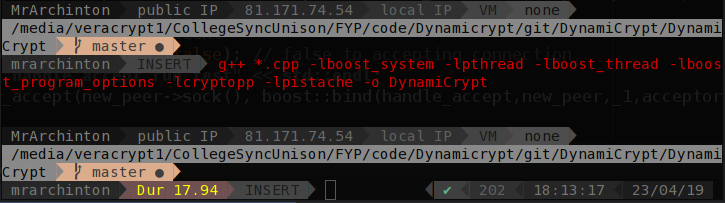
\includegraphics[width=1\textwidth]{Figures/b1.png}
  \caption[Compiling DynamiCrypt]{Compiling DynamiCrypt}
  \label{fig:b1}
\end{figure}
\FloatBarrier

Figure \ref{fig:b1} shows the result of the compilation and as you can see there are no errors or warnings present, this is an indication that the code is syntax correct and operations are performed for the correct data types.

Every program starts of with a main function. DynamiCrypt's main function is rather light, all it does is processes the command line arguments, creates a listening peer and creates the API server object.
To create an initial peer the already seen before code is used.
\begin{lstlisting}
ip::tcp::acceptor acceptor(service, ip::tcp::endpoint(ip::tcp::v4(), listen_port));
peer::ptr initial_peer = peer::new_(false);
acceptor.async_accept(initial_peer->sock(), boost::bind(handle_accept,initial_peer,_1, &acceptor));
\end{lstlisting}
Here an acceptor object is created this allows for the peer object to listen on a port on the localhost.
\begin{lstlisting}
peer::new_(false);
\end{lstlisting}
Is used to notify the peer object that this peer will be waiting for a connection.
\begin{lstlisting}
void handle_accept(peer::ptr peer, const boost::system::error_code & err, ip::tcp::acceptor* acceptor) {
    peer->start("",""); // starts current client
    // creates and listens for new client
    peer::ptr new_peer = peer::new_(false); // false to accepting connection
    //std::cout << "handle_accept run test" << std::endl;
    acceptor->async_accept(new_peer->sock(), boost::bind(handle_accept,new_peer,_1,acceptor)); // this 
}
\end{lstlisting}
The above function is called when the asynchronous connect object receives an external tcp request. The start method is called on the current peer followed by a creation of a new peer which will start listening for the next connection. This way there is always only one peer waiting for new connections. 

Because of how Boost manages asynchronous programming by using a service object to manage threads as well as using the proactor design pattern where asynchronous operations can occur using only one thread. However because DynamiCrypt is operation heavy when it comes to synchronisation I have used both threads and the proactor approach, this way when an asynchronous operation is about to take place Boost will choose a random available thread for it to run on. 
For this reason there are a few operations taking place in the main.cpp file to set all of this up.
\begin{lstlisting}
boost::thread_group threads;

start_listen(4);

void start_listen(int thread_count) {
    for ( int i = 0; i < thread_count; ++i)
        threads.create_thread( listen_thread);
}

void listen_thread() {
    service.run();
}

}
\end{lstlisting}
A group of threads variable is allocated, then the start listen function is called in the main function, this function creates four threads in this case and executes the service.run() function in each thread. This just executes boost asynchronous handler on each of the four threads. 

Finally to ensure a clean exit without leaving any zombie processes the main function will wait for all the threads to finish their execution.
\begin{lstlisting}
threads.join_all();
\end{lstlisting}

The API server is a bit more straight forward since the threads and asynchronous operations are more hidden away from the user by the Pistache library. 
\begin{lstlisting}
api_service_data_handler.set_address_and_port_of_sync("127.0.0.1", listen_port);
APIServer api_server(api_port);
\end{lstlisting}
The first line here sets the address of the sync-server and the port on which it is listening on as this information will be shared with the NodeJs app later. 
The actual creation of the API is simply calling the constructor with a port number.

The API and the sync-server require each other for operation, however it would be confusing if both were explained at the same time therefore the API will be covered initially followed by the sync-server.

\section{API}
The constructor of the API server creates the variables needed for the server and ofloads it to the APIservice object.
\begin{lstlisting}
APIServer::APIServer(int port_number) {
    Pistache::Port port(port_number);
    int thr = 2;
    Pistache::Address addr(Pistache::Ipv4::any(), port);
    //cout << "Cores = " << hardware_concurrency() << endl;
    std::cout << "API Using " << thr << " threads" << std::endl;
    API_service api(addr);
    api.init(thr);
    api.start();
    api.shutdown();
}
\end{lstlisting}
For the API two threads were defined as this is enough to handle multiple clients.
The threads are created as follows.
\begin{lstlisting}
void API_service::init(size_t thr = 2) {
    auto opts = Pistache::Http::Endpoint::options()
        .threads(thr)
        .flags(Pistache::Tcp::Options::InstallSignalHandler);
    httpEndpoint->init(opts);
    createDescription();
}
\end{lstlisting}
Pistache is a much more high level library than Boost therefore for the setup I mostly followed the examples they have in their GitHub repository.
\begin{lstlisting}
void API_service::start() {
    router.initFromDescription(desc);
    httpEndpoint->setHandler(router.handler());
    httpEndpoint->serve();
}
\end{lstlisting}
start() sets up the description which in Pistache's case is the information about all the routes available, some licensing and API info.  

Here is a small extract from the function that creates the description
\begin{lstlisting}
void API_service::createDescription() {
    desc
        .info()
        .license("Apache", "http://www.apache.org/licenses/LICENSE-2.0");

    auto backendErrorResponse =
        desc.response(Pistache::Http::Code::Internal_Server_Error, "An error occured with the backend");

    desc
        .schemes(Pistache::Rest::Scheme::Http)
        .basePath("/v1")
        .produces(MIME(Application, Json))
        .consumes(MIME(Application, Json));

    auto versionPath = desc.path("/v1");

    auto path = versionPath.path("/options");

    path
        .route(desc.get("/test-ok"))
        .bind(&API_service::route_test, this)
        .produces(MIME(Application, Json), MIME(Application, Xml))
        .response(Pistache::Http::Code::Ok, "ok");
    
    path
        .route(desc.post("/init"), "Initiate Communication")
        .bind(&API_service::initial, this)
        .produces(MIME(Application, Json))
        .consumes(MIME(Application, Json))
        .response(Pistache::Http::Code::Ok, "Initial request")
        .response(backendErrorResponse);
\end{lstlisting}
The path is built by firstly specifying the version of the API this way it is possible to support legacy code using you old API. Next I decided to put all the DynamiCrypt operations preceded by /options this way in the future if the API can be expanded to do other things like maybe formatting / encoding data. Next is the actual routes used by the DynamiCrypt API. The first one is /test-ok a GET route, this is handy if you want to check if the API is up and running. To access this route you would send a get request to this for example 127.0.0.1:9081/v1/options/test-ok/. This simple route will just return "ok" as can be seen when a curl get request is being made as can be seen in figure \ref{fig:b2}.

\begin{figure}[!h]
  \centering
      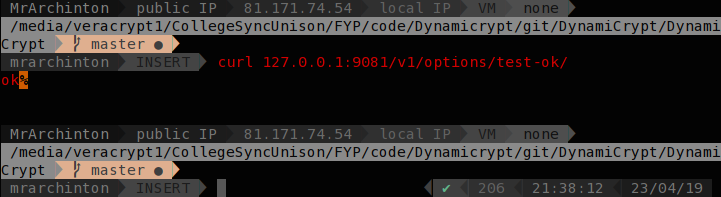
\includegraphics[width=1\textwidth]{Figures/b2.png}
  \caption[127.0.0.1:9081/v1/options/test-ok/]{127.0.0.1:9081/v1/options/test-ok/}
  \label{fig:b2}
\end{figure}
\FloatBarrier

The list of all routes currently available in the API and a brief description are as follows.
\begin{lstlisting}
/v1/options/test-ok         GET
// test if API is up
/v1/options/init            POST
// Initial request
/v1/options/init_config     POST
// Initial Config
/v1/options/sync            POST
// Begin Sync
/v1/options/status          POST
// check if connected to tpm ok
/v1/options/encrypt         POST
// encrypt / decrypt data
/v1/options/exit            POST
// delete tpm and data associated with the app using the API
/v1/options/:rest           POST
// custom 404
\end{lstlisting}

Every post route is handled by a specific function.
\begin{lstlisting}
 path
        .route(desc.post("/init"), "Initiate Communication")
        .bind(&API_service::initial, this)
        .produces(MIME(Application, Json))
        .consumes(MIME(Application, Json))
        .response(Pistache::Http::Code::Ok, "Initial request")
        .response(backendErrorResponse);
\end{lstlisting}

In this case every time the init route is called the initial() function handles it and produces its own response. Here is the initial function bellow.

\begin{lstlisting}
void API_service::initial(const Pistache::Rest::Request& request, Pistache::Http::ResponseWriter response) {
    rapidjson::Document document;
    // make into json object
    char * jsonBody = new char [request.body().length()+1];
    strcpy (jsonBody, request.body().c_str());
    document.Parse(jsonBody);
    
    std::string service_name;
    int data_ok = 1;

    if(document.HasMember("service_name")){
        if(document["service_name"].IsString()){
            service_name = document["service_name"].GetString();
        }
        else{
            data_ok = 0;
        }
    }
    else{
        data_ok = 0;
    }
    
    std::string respond_service_name;
    rapidjson::StringBuffer buffera;
    rapidjson::Writer<rapidjson::StringBuffer> writera(buffera);
    
    if(data_ok){
        respond_service_name = api_service_data_handler.new_service(service_name);
        writera.StartObject(); 
        writera.Key("service_name");                
        writera.String(respond_service_name.c_str(), respond_service_name.length());
        writera.Key("address_of_this_tpm");                
        writera.String(api_service_data_handler.get_sync_address().c_str(), api_service_data_handler.get_sync_address().length());
        writera.Key("port_of_this_tpm");
        writera.Uint(api_service_data_handler.get_sync_port());
        writera.EndObject();
        
    }
    
    else{//error with request
        writera.StartObject(); 
        writera.Key("error");                
        writera.String("invalid request");
        writera.EndObject();
    }
    
    response.send(Pistache::Http::Code::Ok, buffera.GetString());
}
\end{lstlisting}

Similar to NodeJs each of these handlers have a reference to a request and response object.
For extracting JSON data the RapidJson library is used, it is also used for creating JSON data.
The API interacts with the 
\begin{lstlisting}
api_service_data_handler
\end{lstlisting} 
object for managing the services.

It will take too long to go through all of the routes and how they function so a more basic explanation will suffice. I would recommend watching my demo video here https://www.youtube.com/watch?v=LsR4XsGrDCY&feature=youtu.be 
on YouTube as it would be easier to understand.

Initially the NodeJs apps must register with the API this unfortunately turned out to be a multi step process however it is necessary since the API needs data from both of the Apps that wish to use DynamiCrypt.

\begin{figure}[!h]
  \centering
      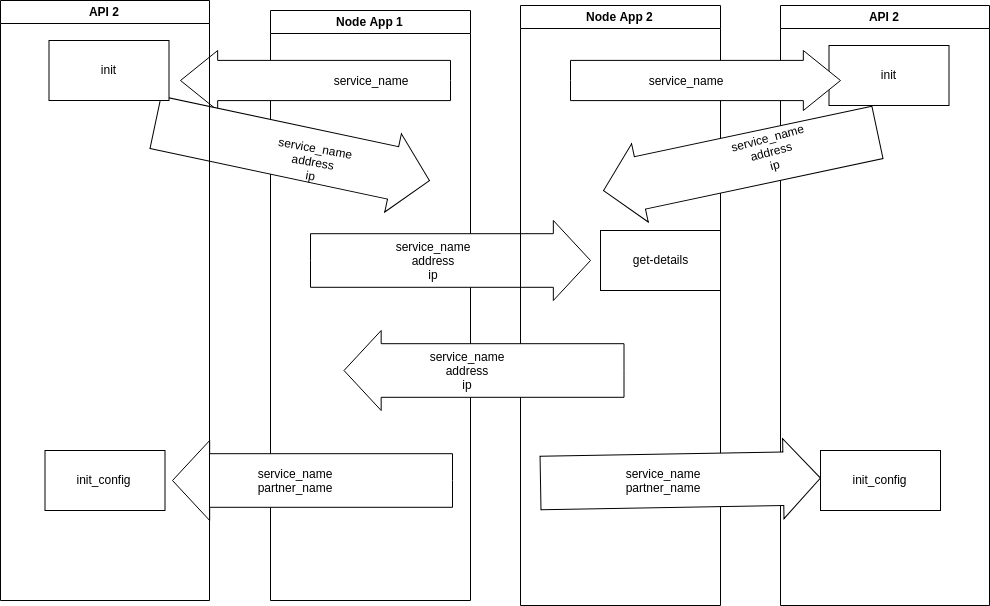
\includegraphics[width=1\textwidth]{Figures/connect_code_flow.png}
  \caption[How Node Apps register with the API]{How Node Apps register with the API}
  \label{fig:b3}
\end{figure}
\FloatBarrier

Figure \ref{fig:b3} is a call flow diagram of how the NodeJS apps register themselves with the API.
The same can be demonstrated by using Wireshark and listening on localhost. The filters I used are (tcp.port == 9081) && http since I only want to see POST requests for the API running on port 9081 since the POST requests for the other API are identical so there is no point in showing it twice.

\begin{figure}[!h]
  \centering
      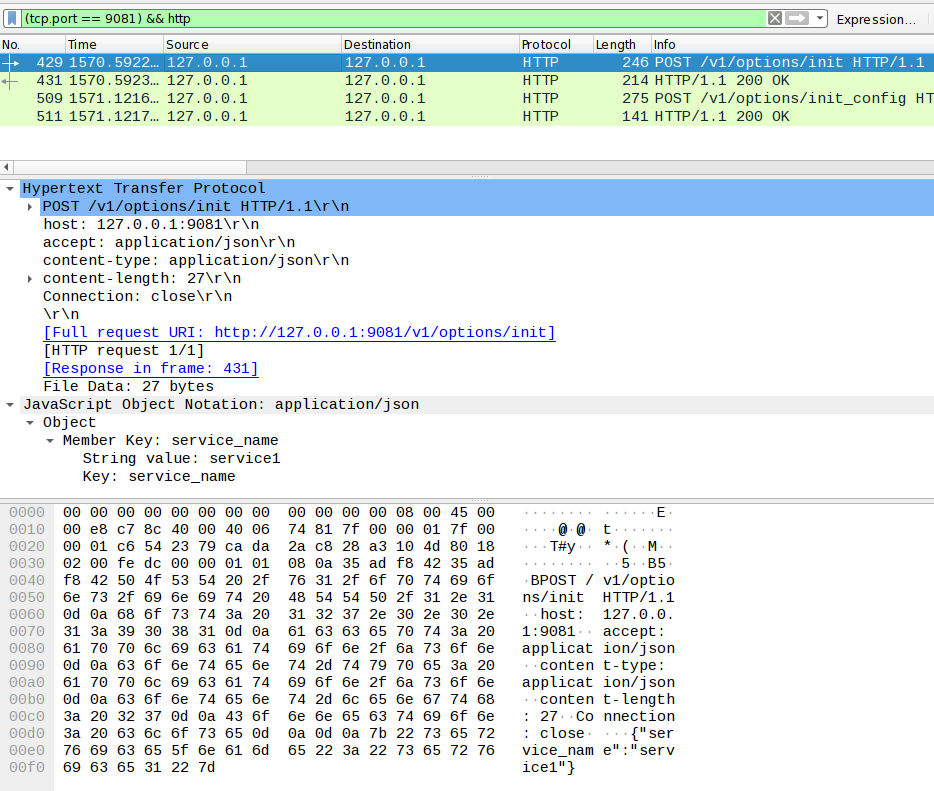
\includegraphics[width=1\textwidth]{Figures/b4.png}
  \caption[POST request to init]{POST request to init}
  \label{fig:b4}
\end{figure}
\FloatBarrier
Figure \ref{fig:b4} shows how the NodeJs App sent a POST request to the init route with its user service name. 

\begin{figure}[!h]
  \centering
      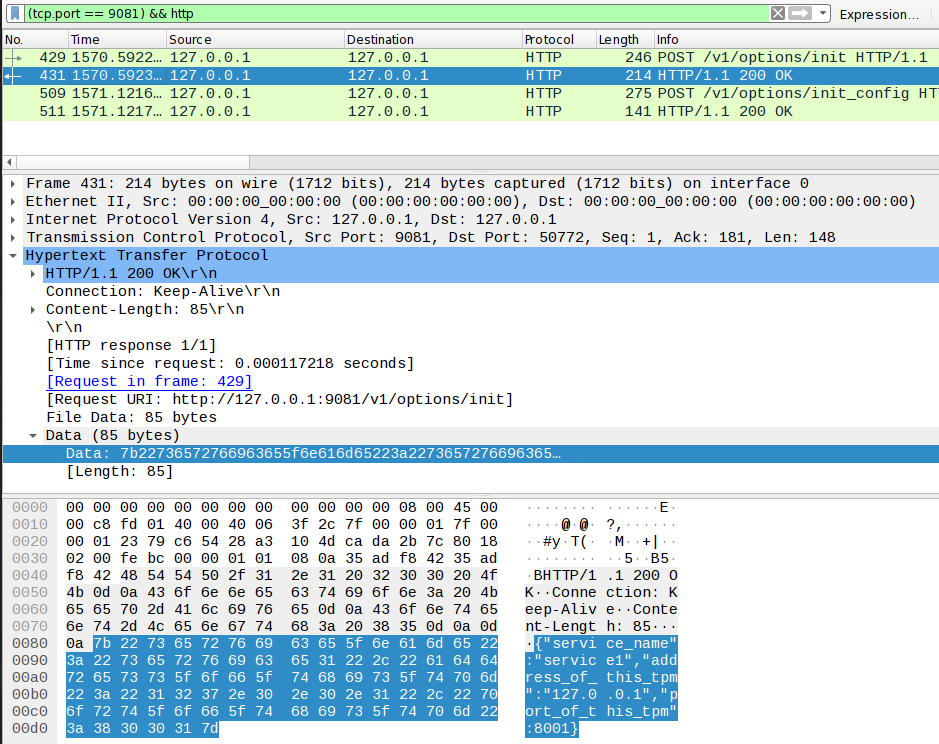
\includegraphics[width=1\textwidth]{Figures/b5.png}
  \caption[API response]{API response}
  \label{fig:b5}
\end{figure}
\FloatBarrier
Figure \ref{fig:b5} shows how the APIs reply to the previous post request with the service name the API wants the NodeJS App to use, the port of the sync-server and the address of the sync-server.
After this the Node App would make a request to the other Node App for the get details route to exchange information. This can also be acquired with Wireshark by changing a filter as seen in figure \ref{fig:b8}.
\begin{figure}[!h]
  \centering
      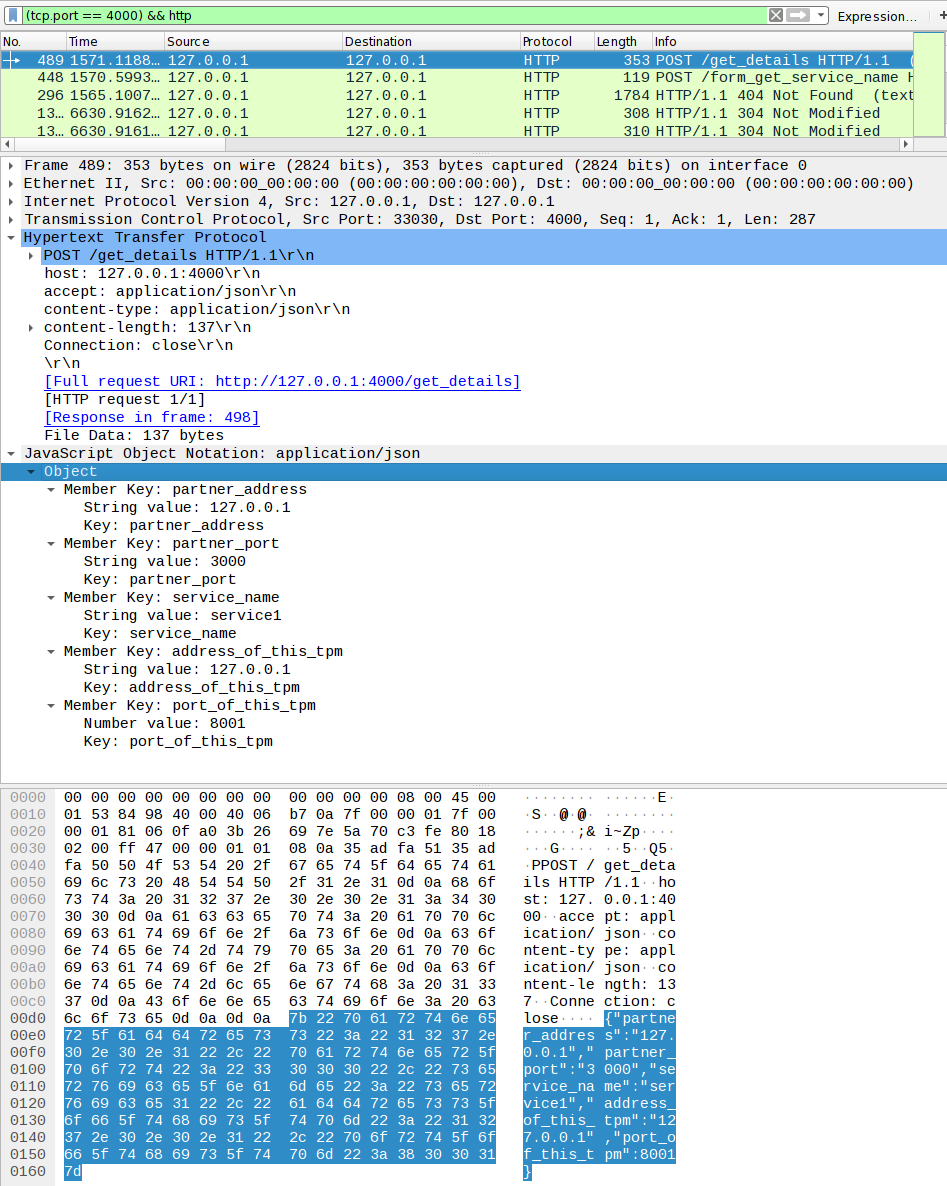
\includegraphics[width=1\textwidth]{Figures/b8.png}
  \caption[POST request to other NodeJs app's get details route]{POST request to other NodeJs app's get details route}
  \label{fig:b8}
\end{figure}
\FloatBarrier


\begin{figure}[!h]
  \centering
      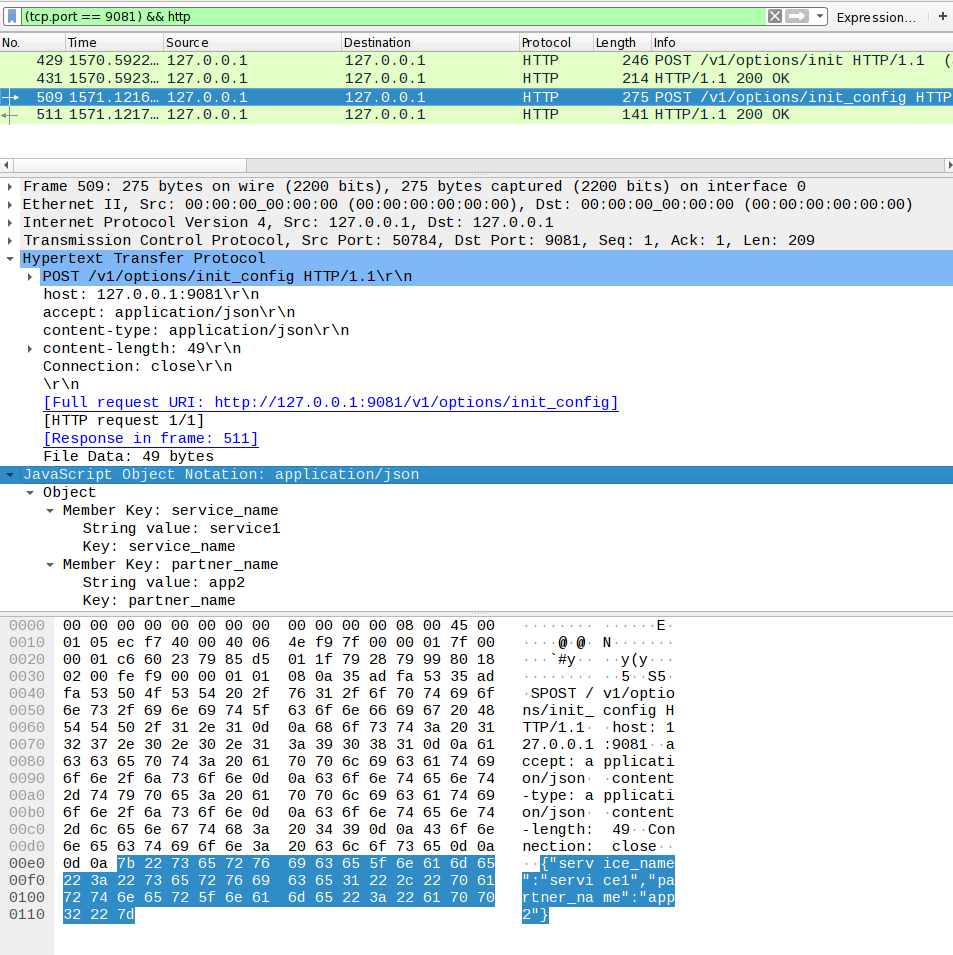
\includegraphics[width=1\textwidth]{Figures/b6.png}
  \caption[POST request to init config]{POST request to init config}
  \label{fig:b6}
\end{figure}
\FloatBarrier
Figure \ref{fig:b6} shows how the NodeJs app updates the API with the service name of the other NodeJs app in this case it is called partner name.

\begin{figure}[!h]
  \centering
      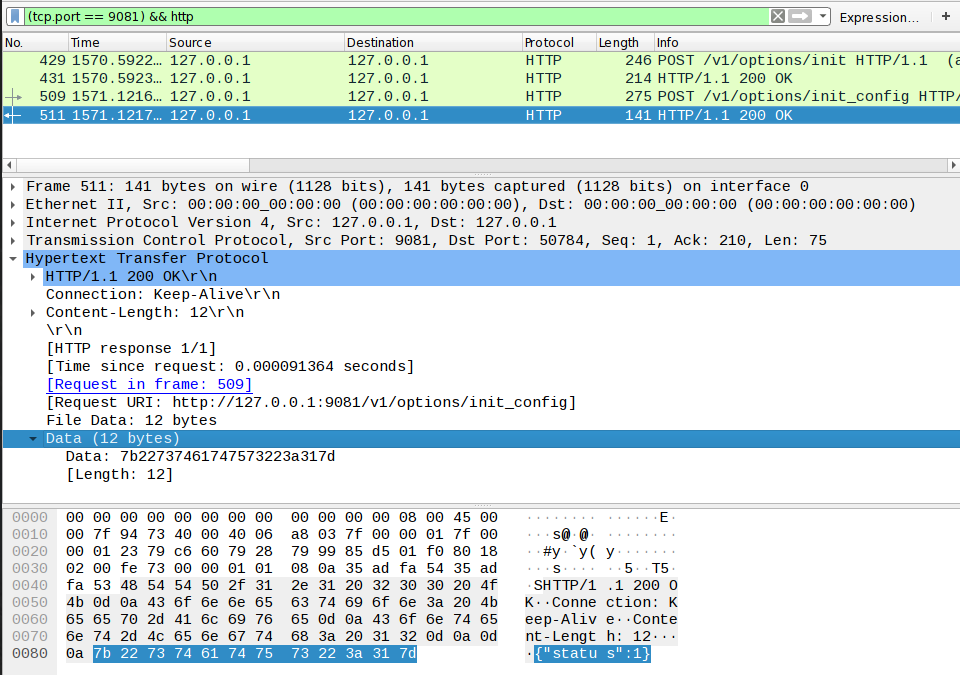
\includegraphics[width=1\textwidth]{Figures/b7.png}
  \caption[API response]{API response}
  \label{fig:b7}
\end{figure}
\FloatBarrier
Figure \ref{fig:b7} shows the APIs reply to the previous post request with a status 1 which means everything is OK and the update was successfully made.
Now the two NodeJs apps are fully registered with the API. The next step is to tell the API to tell the sync-server to start synchronising so that the Apps can send messages to each other using dynamic encryption.
For this to occur one of the Apps must simply call the sync route of the API.

\begin{figure}[!h]
  \centering
      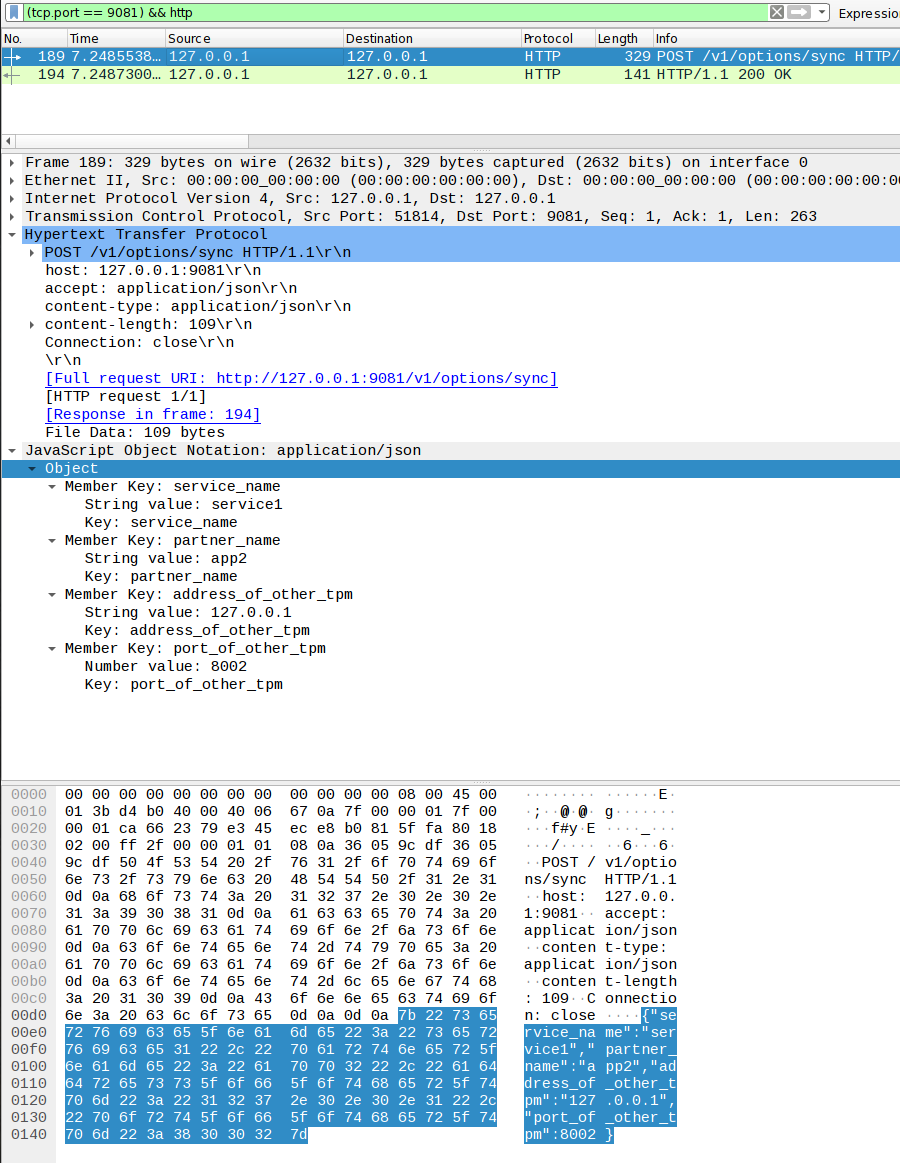
\includegraphics[width=1\textwidth]{Figures/b9.png}
  \caption[POST request to sync]{POST request to sync}
  \label{fig:b9}
\end{figure}
\FloatBarrier
Figure \ref{fig:b9} shows the sync route of the API is called. The Node App sends a lot of details this time including service name, partner name, the address and port of the sync-server that is used by the other API that the other NodeJs App communicates with. This is because it is calling a different function outside of the api service data handler object. This time a function from the definitions.cpp is called.
\begin{lstlisting}
int begin_sync(std::string address, int port, std::string service_name, std::string partner_name){
    try{
        peer::ptr initiating_peer = peer::new_(true, address, port);
        initiating_peer->start(service_name, partner_name);
    }
    catch(std::exception& e){
        return 0;
    }
    return 1;
}
\end{lstlisting} 
Here a new peer is created of connecting type instead of listening type like we looked at last time. This peer will try to connect to the sync-server at the address and port the Node App sent it.

\begin{figure}[!h]
  \centering
      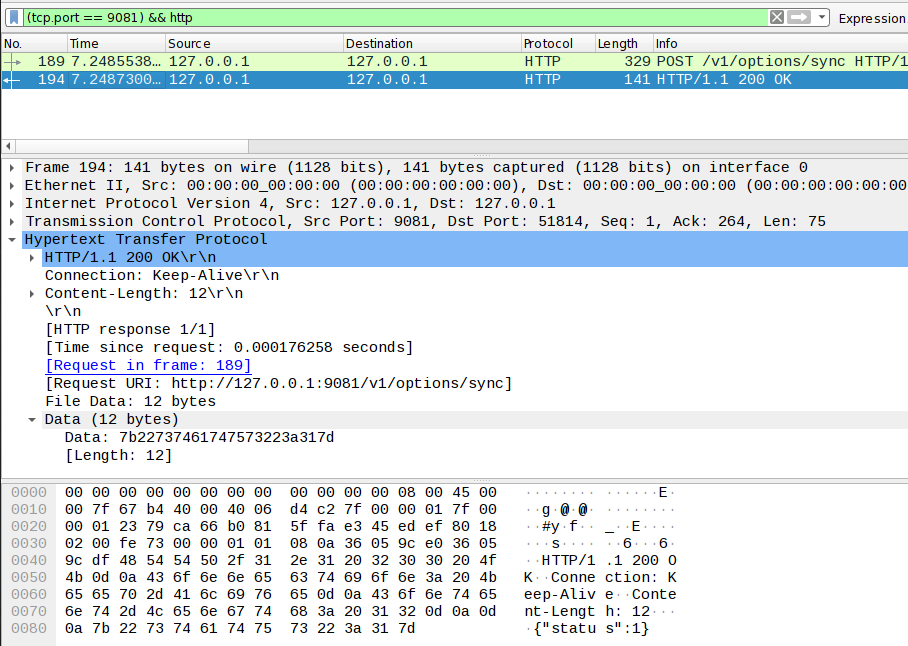
\includegraphics[width=1\textwidth]{Figures/b10.png}
  \caption[API response]{API response}
  \label{fig:b10}
\end{figure}
\FloatBarrier
Figure \ref{fig:b10} shows the APIs reply to the previous post request with a status 1 which means the request was processed successfully however this does not mean that the sync-server connected to the other sync-server correctly this is because of the asynchronous nature of the sync-server it is impossible to get the result of the connection. Therefore the NodeJs app should query the API to see if the connection was successful and if the two sync-servers are currently syncing this is done by calling the status route in the API and providing the service name. if the status returned is 1 then the two sync-servers are currently synchronising, if the status is 0 then they failed to connect or some other error occurred.

\textbf{Encryption / Decryption}

Now the NodeJs apps can send messages to the API to be encrypted.
How encryption works is it selects the appropriate key from the key store based on the mode provided.
The key store looks like this.
\begin{lstlisting}
struct key_store {
    std::string key;
    int uses;
};

struct API_data {
    std::string service_name_;
    std::string service_name_partner_;
    std::vector<key_store> keys_;
};
\end{lstlisting} 
This is an inner struct inside the 
\begin{lstlisting}
API_service_data_handler
\end{lstlisting} 
class which contains a vector of API data objects.

Currently DynamiCrypt supports two encryption methods. Encryption mode 1 will simply use the latest key avaiable in the keystore, this mode is handy if you want the fastest mode of encryption available.
For encryption mode 1, 
\begin{lstlisting}
if(mode == 1){
                //check for any latest key 
                if(api_data->keys_.size() == 0){
                    return DYNAMICRYPT_API_WAIT;
                }else{
                    string_key = api_data->keys_.back().key;
                    api_data->keys_.back().uses ++;
                    if(PRINT_API_CRYPT_MESSAGES){
                        std::cout << "got key like this " << string_key << std::endl;
                        std::cout << "key was used " << api_data->keys_.back().uses << " times" << std::endl;
                    }
                }
            
            }
\end{lstlisting} 
The appropriate api data object is selected referring to the service that called the API.
The size of the key store is initially checked to see if it contains any keys, if not then the API will tell the Node App to wait. The node app can then query the API again and again for encryption or just use a timeout and wait for 100 milliseconds or so. 
If there is keys in the key store then the last key that was entered is used for encryption. The uses count of this particular key is also increased, the uses count doesn't really matter for mode 1 but will matter for mode 2 and future modes that are not implemented yet. 

Encryption mode 2 would be the more secure one as only keys that have 0 uses are picked this way each message would be encrypted using its own unique key.
\begin{lstlisting}
else if (mode == 2){
                if(api_data->keys_.size() == 0){
                    return DYNAMICRYPT_API_WAIT;
                }
                else{
                    int attempts_to_find_key = 0; //search max_attempts_to_decrypt times for the key since decrypt will only search for max_attempts_to_decrypt times too
                    int found_key = 0;
                    for(int number_of_keys = api_data->keys_.size()-1; number_of_keys >= 0; number_of_keys --){
                        if(attempts_to_find_key == max_attempts_to_decrypt){
                            break;
                        }
                        attempts_to_find_key ++;
                        if(api_data->keys_.at(number_of_keys).uses == 0){
                            string_key = api_data->keys_.at(number_of_keys).key;
                            api_data->keys_.at(number_of_keys).uses++;
                            if(PRINT_API_CRYPT_MESSAGES){
                                std::cout << "got key like this " << string_key << std::endl;
                                std::cout << "key was used " << api_data->keys_.at(number_of_keys).uses << " times" << std::endl;
                            }
                            found_key = 1;
                            break;
                        }
                    }
                    if(!found_key){
                        return DYNAMICRYPT_API_WAIT;
                    }
                }
            }
\end{lstlisting} 
This mode is a little bit more involved then the simple get latest key. The Basic premise here is to find a suitable key that has 0 uses. This key is found by working back from the latest key down the vector until either a key is found, either the number of keys runs out or the search limit is reached. in this case the search limit is defined at 10 and stored at this variable.
\begin{lstlisting}
max_attempts_to_decrypt
\end{lstlisting} 
This means that in order to find a key provided the key store is longer than 10 the search will max out at 10 elements from the latest. 
This limit is set not so much for encryption but rather the decryption, this is because if there was no limit the encryption algorithm might choose a key that is say 200 keys away from the latest, the decryption algorithm will then have a heck of a time trying to find that correct key to use. 
And just like before if an appropriate key is not found the API will tell the Node App to wait.

After these two algorithms find the appropriate key the next step is to encrypt the data.
\begin{lstlisting}
CryptoPP::byte key[ CryptoPP::AES::MAX_KEYLENGTH ];
gen_key(string_key,key);
std::string for_encode = encrypt(message, key, iv);
\end{lstlisting} 
Earlier I said that the key generated by the tree parity machines will be used to encrypt the message. This is technically not true since that key is actually used to generate the actual key used for encryption. This is because the key generated by the tree parity machines is too long for AES-256 encryption therefore the gen key function generates an appropriate size key without loosing any data, this means that it does not simply cut of the rest of the key that's longer than 32 bytes needed for AES-256. Here is a snippet from that function.
\begin{lstlisting}
void API_service_data_handler::gen_key(std::string string_key, CryptoPP::byte* key){
    if(string_key.length() > CryptoPP::AES::MAX_KEYLENGTH){
            int count_first = 0;
            int count_last = string_key.length() -1;
            int number_of_operations = count_last - CryptoPP::AES::MAX_KEYLENGTH;
            for(int i = 0; i< number_of_operations; i++){
                string_key[count_first] = string_key.at(count_first) + string_key.at(count_last);
                if(count_first == CryptoPP::AES::MAX_KEYLENGTH){
                    count_first = 0;
                }
                count_first ++;
                count_last --;
            }
        }
        
        int string_count = 0;
        for(int i=0; i<CryptoPP::AES::MAX_KEYLENGTH; i++){
            if(string_count == string_key.length() -1){
                string_count = 0;
            }
            key[i] = string_key.at(string_count);
            string_count ++;
        } 
\end{lstlisting} 

After encrypting the data, the ciphertext is then encoded with base 64 encoding. Encoding is necessary because random bytes tend to mess up the structure of the JSON object.
\begin{lstlisting}
std::string encoded = encode_base64(for_encode);
output = encoded;
\end{lstlisting} 

Finally when sending the ciphertext to the node app the API also generates a hash specifically SHA 256 of the original plaintext. this will help the API to determine if the message was decrypted successfully by comparing hashes. Hashes are one way function so it is save to create a hash of the plaintext. The node app would then essentially just forward the ciphertext and the hash to the other node app for decrypting.

Decryption has algorithms specific for each mode therefore decryption mode 1 will directly be capable of decrypting encryption mode 1 and so on. The decryption is a potentially much more operation heavy operation that encryption. This is because it takes a guess at the key then tries to decrypt it and if that fails takes a guess at another key. This might seen pretty bad but from testing normally it only takes one to three decryption attempts to decrypt the key since the most likely key would be the latest one.

The decryption section of the code initially decodes the data from base 64 then that data is passed to the various decryption algorithms based on the mode.

For decryption mode 1
\begin{lstlisting}
if(mode == 1){
                if(api_data->keys_.size() == 0){
                    return DYNAMICRYPT_API_WAIT; // no keys in key ring shouldn't happen with decrypt if used properly
                }
                int number_of_keys = api_data->keys_.size()-1;  // maybe change to keys_.size()-1
                for(int decrypt_loop = 0; decrypt_loop<max_attempts_to_decrypt; decrypt_loop++){
                    //try last key first
                    std::string string_key = api_data->keys_.at(number_of_keys).key;
                    if(PRINT_API_CRYPT_MESSAGES){
                        std::cout << "trying to decrypt with key " << string_key << std::endl;
                        std::cout << "key was used " << api_data->keys_.at(number_of_keys).uses << " times" << std::endl;
                    }
                    CryptoPP::byte key[ CryptoPP::AES::MAX_KEYLENGTH ];
                    gen_key(string_key,key);

                    output = decrypt(decoded_message, key, iv);
                    if(!hash_with_sha_256(output).compare(hash)){ //decrypted successfully
                        api_data->keys_.at(number_of_keys).uses ++;
                        break;
                    }

                    if(number_of_keys == 0){
                        //output = "failed";
                        return DYNAMICRYPT_API_FAILED_DECRYPT;
                        break;
                    }

                    number_of_keys --;
                
                }
            }
\end{lstlisting} 
This checks if there are keys in the key ring this is not necessary since the tree parity machines generate the same keys at pretty much the same time but it is just in there as a sanity check or to catch some other strange errors. This is because for decryption the key is presumed to exist since that key was used to encrypt in the first place.

Since this is mode 1 we can simply try the latest key first then work down from there. Again how much further down you can go depends on the size of the key store and the limitation put in place to prevent traversing all the keys in case of an error or broken data.

Next the message is decrypted and hashed and the hash is compared to the hash sent by the node app. if the hashes match then the plaintext is returned if not the next key in line is tested.
If the hashes match the uses for the key is incremented this is important because you don't want this API using the same key for encryption as the other API if using mode 2. 
In the unlikely event that all the keys tried failed to decrypt the message a failure message will be sent to the node App, during testing I never have seen this scenario occur however it is likely to happen if you delay sending the encrypted data for decryption by quite some time like ten or more seconds since the key store will be filled up with new keys and the old key required for decryption will be pushed back past the limit. For this reason it is important for the node apps to send the ciphertext to the other node app as soon as possible.

For decrypting mode 2 quite a long algorithm is used. 
\begin{lstlisting}
else if (mode == 2){ // try keys with 0 uses first
                std::string string_key;
                if(api_data->keys_.size() == 0){
                    return DYNAMICRYPT_API_WAIT; // no keys in key ring shouldn't happen with decrypt if used properly
                }
                int has_skipped_keys = 0;
                int number_of_keys = api_data->keys_.size()-1;  // maybe change to keys_.size()-1
                
                //std::cout << "number_of_keys at start " << number_of_keys << std::endl;
                std::vector<int> skipped_keys;
                for(int decrypt_loop = 0; decrypt_loop<max_attempts_to_decrypt; decrypt_loop++){
                    //std::cout << "decrypt_loop at start " << decrypt_loop << std::endl;
                    if(number_of_keys == -1){ // needed because of the continue which could cause number_of_keys to be -1
                        break;
                    }
                    
                    if(api_data->keys_.at(number_of_keys).uses == 0){
                        
                        string_key = api_data->keys_.at(number_of_keys).key;
                        //std::cout << "key with 0 uses found " << string_key << std::endl;
                    }else{
                        skipped_keys.push_back(number_of_keys);
                        //std::cout << "skipping key at index " << number_of_keys << std::endl;
                        number_of_keys --;
                        has_skipped_keys = 1;
                        
                        continue;
                    }
                    
                    if(PRINT_API_CRYPT_MESSAGES){
                        std::cout << "trying to decrypt with key " << string_key << std::endl;
                        std::cout << "key was used " << api_data->keys_.at(number_of_keys).uses << " times" << std::endl;
                    }
                    CryptoPP::byte key[ CryptoPP::AES::MAX_KEYLENGTH ];
                    gen_key(string_key,key);

                    output = decrypt(decoded_message, key, iv);
                    if(!hash_with_sha_256(output).compare(hash)){ //decrypted successfully
                        api_data->keys_.at(number_of_keys).uses ++;
                        return output;
                    }

                    if(number_of_keys == 0){
                        break;
                    }

                    number_of_keys --;
                
                }
                //code runs here only if decryption was unsuccessful
                if(has_skipped_keys){ //check for skipped keys
                    for(int i = 0; i < skipped_keys.size(); i ++ ){
                        string_key = api_data->keys_.at(i).key;
                        if(PRINT_API_CRYPT_MESSAGES){
                            std::cout << "trying to decrypt with key " << string_key << std::endl;
                            std::cout << "key was used " << api_data->keys_.at(i).uses << " times" << std::endl;
                        }
                        CryptoPP::byte key[ CryptoPP::AES::MAX_KEYLENGTH ];
                        gen_key(string_key,key);

                        output = decrypt(decoded_message, key, iv);
                        if(!hash_with_sha_256(output).compare(hash)){ //decrypted successfully
                            api_data->keys_.at(i).uses ++;
                            return output;
                        }
                    }
                    // if key not decrypted then code is continued here therefore
                    //output = "failed";
                    return DYNAMICRYPT_API_FAILED_DECRYPT;
                }else{
                    //output = "failed";
                    return DYNAMICRYPT_API_FAILED_DECRYPT;
                }

            }
\end{lstlisting} 
The reason this is quite long is because of the introduction of skipped keys. Because for encryption mode 2 we only use a key with 0 uses. Therefore to speed up decryption we can test all the keys within the limit that have 0 uses since keys with 0 uses are most likely to decrypt the message for mode 2. 
If the keys with 0 uses fail to decrypt then the keys with more than 0 uses are that were skipped are tested, this should not happen but due to network latency it can be possible where both of the node apps send an encrypt request with mode 2 at the same time and the API manages to use the same key for both, this is very unlikely however just in case it does the code can take care of this scenario, and adding code here doesn't decrease the performance at all since it is just an if statement wouldn't even be called because of the break if the keys with 0 uses successfully decrypted the message. 

Now that we have an idea of how the encryption / decryption operates its time to demonstrate it in action.
I will use the quick setup python script to register the node apps quickly. The quick setup simply "fills out the forms" via code rather than hand. The script looks like this and is included in the Github repository.
\begin{lstlisting}
#!/usr/bin/env python3.7

import requests
import time

Service_one_name = "service1"
Service_two_name = "app2"

Service_one_address = "127.0.0.1"
Service_one_port = 3000

Service_two_address = "127.0.0.1"
Service_two_port = 4000

Service_one_API_address = "127.0.0.1"
Service_two_API_address = "127.0.0.1"

Service_one_API_port = 9081
Service_two_API_port = 9082


url1 = "http://" + Service_one_address + ":" + str(Service_one_port) + "/form_get_service_name"
data = {'Service_name':Service_one_name, 'API_port': Service_one_API_port, 'API_Address': Service_one_API_address} 

r = requests.post(url = url1, data = data) 


url1 = "http://" + Service_two_address + ":" + str(Service_two_port) + "/form_get_service_name"
data = {'Service_name':Service_two_name, 'API_port': Service_two_API_port, 'API_Address': Service_two_API_address} 

r = requests.post(url = url1, data = data) 

time.sleep(0.5)

# now send info to parnter
url2 = "http://" + Service_one_address + ":" + str(Service_one_port) + "/form_send_to_partner"
data = {'port': Service_two_port, 'address': Service_two_address} 
r = requests.post(url = url2, data = data) 

# can now press sync in the browser
\end{lstlisting}

\begin{figure}[!h]
  \centering
      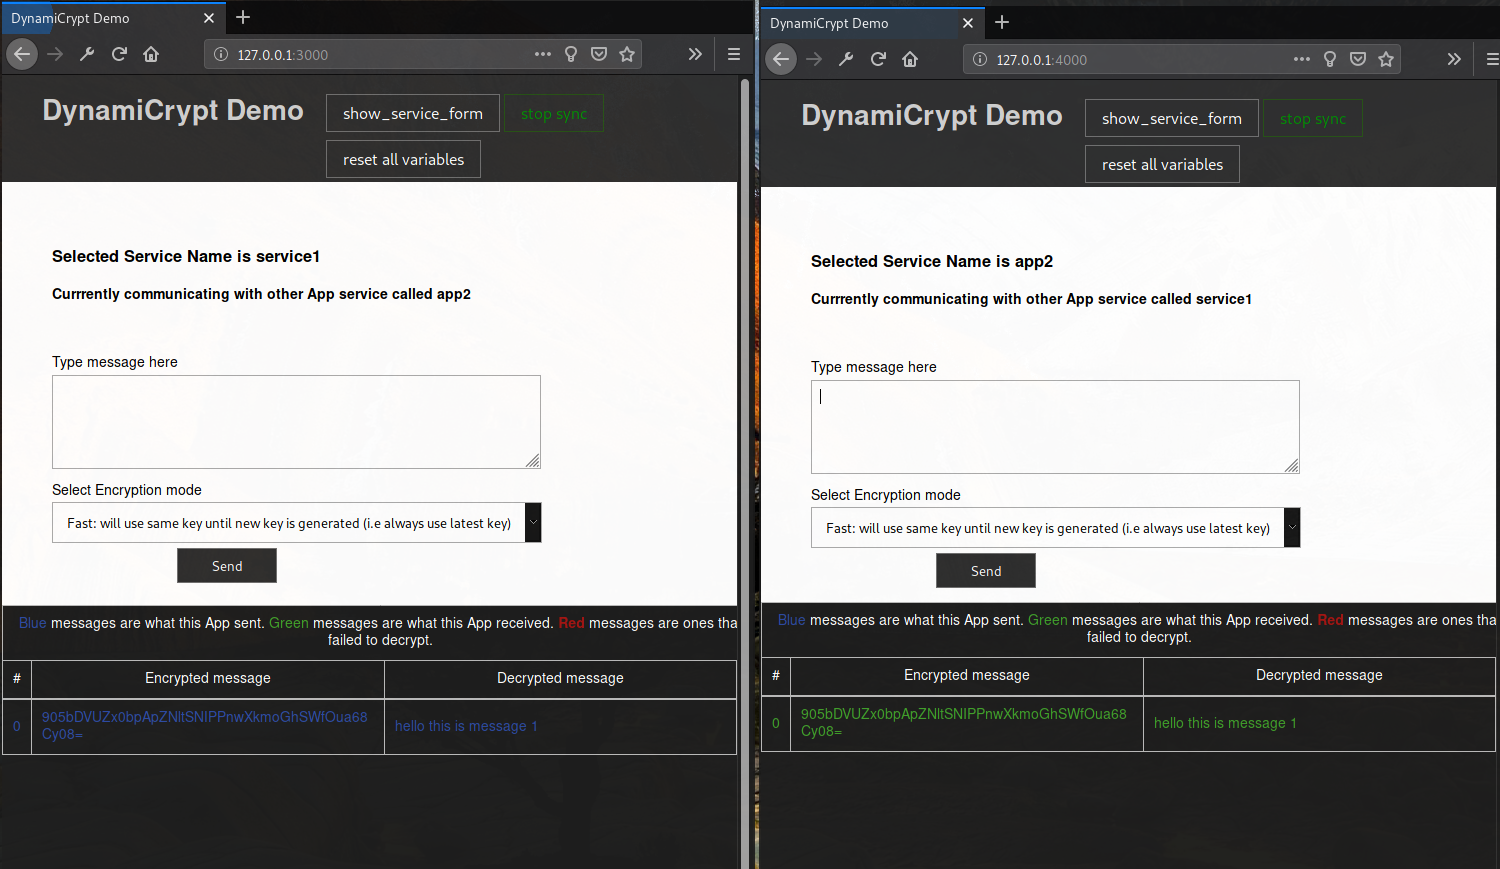
\includegraphics[width=1\textwidth]{Figures/b13.png}
  \caption[Encryption Node App view]{Encryption Node App view}
  \label{fig:b13}
\end{figure}
\FloatBarrier

Figure \ref{fig:b13} shows the two node Apps after a message "hello this is message 1" was sent using the text box interface of the left App. As you can see the right node App decrypted the text successfully.
I will use Wireshark once again to show the data sent between the Node Apps and the API.

\begin{figure}[!h]
  \centering
      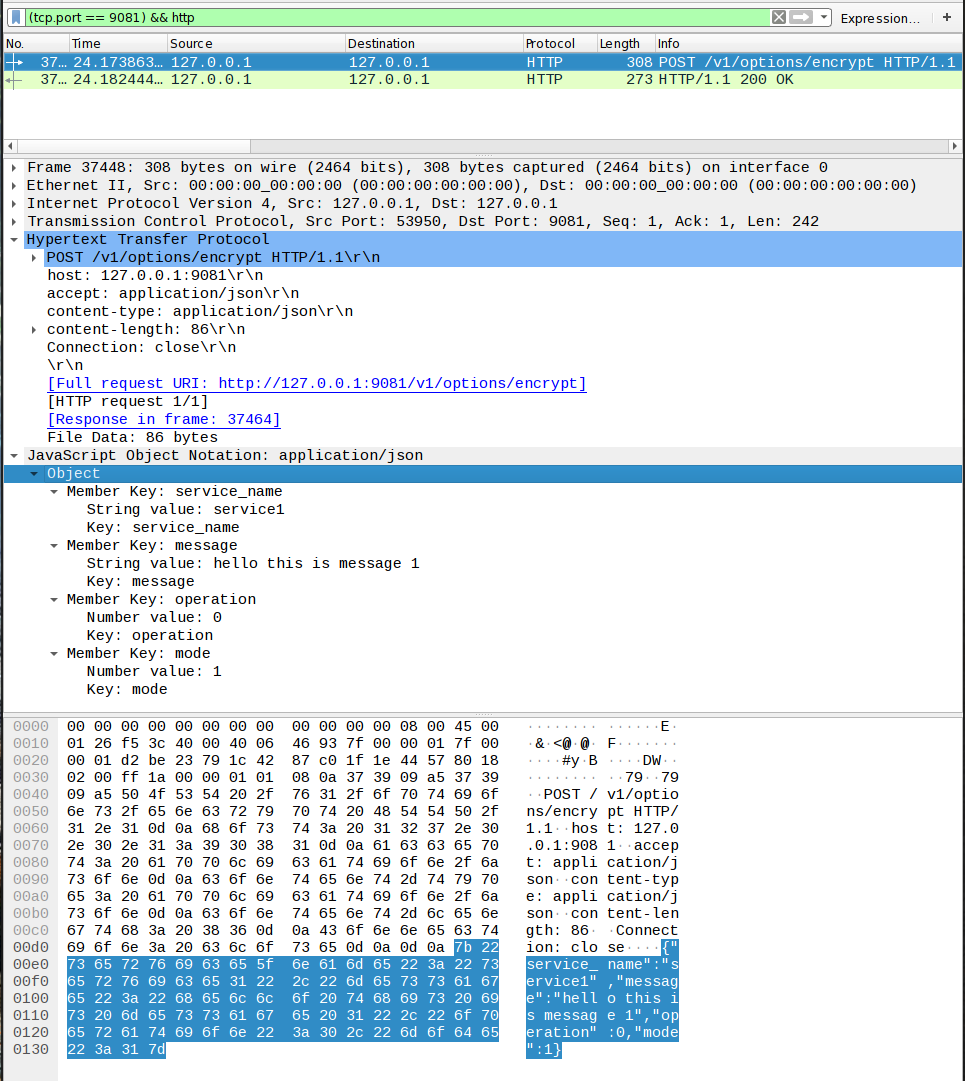
\includegraphics[width=1\textwidth]{Figures/b11.png}
  \caption[Node sends encryption message to the API ]{Node sends encryption message to the API}
  \label{fig:b11}
\end{figure}
\FloatBarrier
Figure \ref{fig:b11} shows the node app at port 3000 sending a post request to the encrypt route of the API.
The data it sends are as follows, service name so the API can identify which key store is appropriate for this service, message the plaintext that will be encrypted, operation this just means whether to encrypt or decrypt because the same route is used, in this case it is 0 but for decryption it would be 1. And finally the encryption mode, mode 1 was chosen in this case.

\begin{figure}[!h]
  \centering
      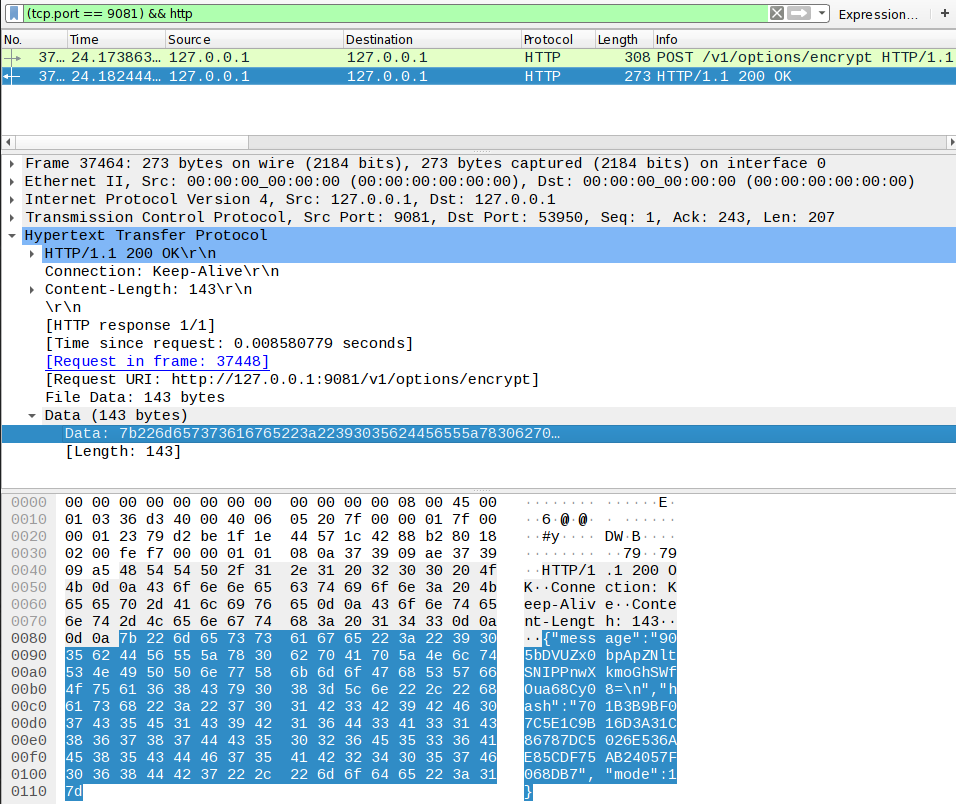
\includegraphics[width=1\textwidth]{Figures/b12.png}
  \caption[API responds with ciphertext and hash]{API responds with ciphertext and hash}
  \label{fig:b12}
\end{figure}
\FloatBarrier
Figure \ref{fig:b12} shows the response of the API, the API replies with the ciphertext as the message, followed by the hash of the plaintext and the mode to be used for decryption. This data will then be forwarded to the other node App by posting it to its decrypt route as seen in figure \ref{fig:b16}


\begin{figure}[!h]
  \centering
      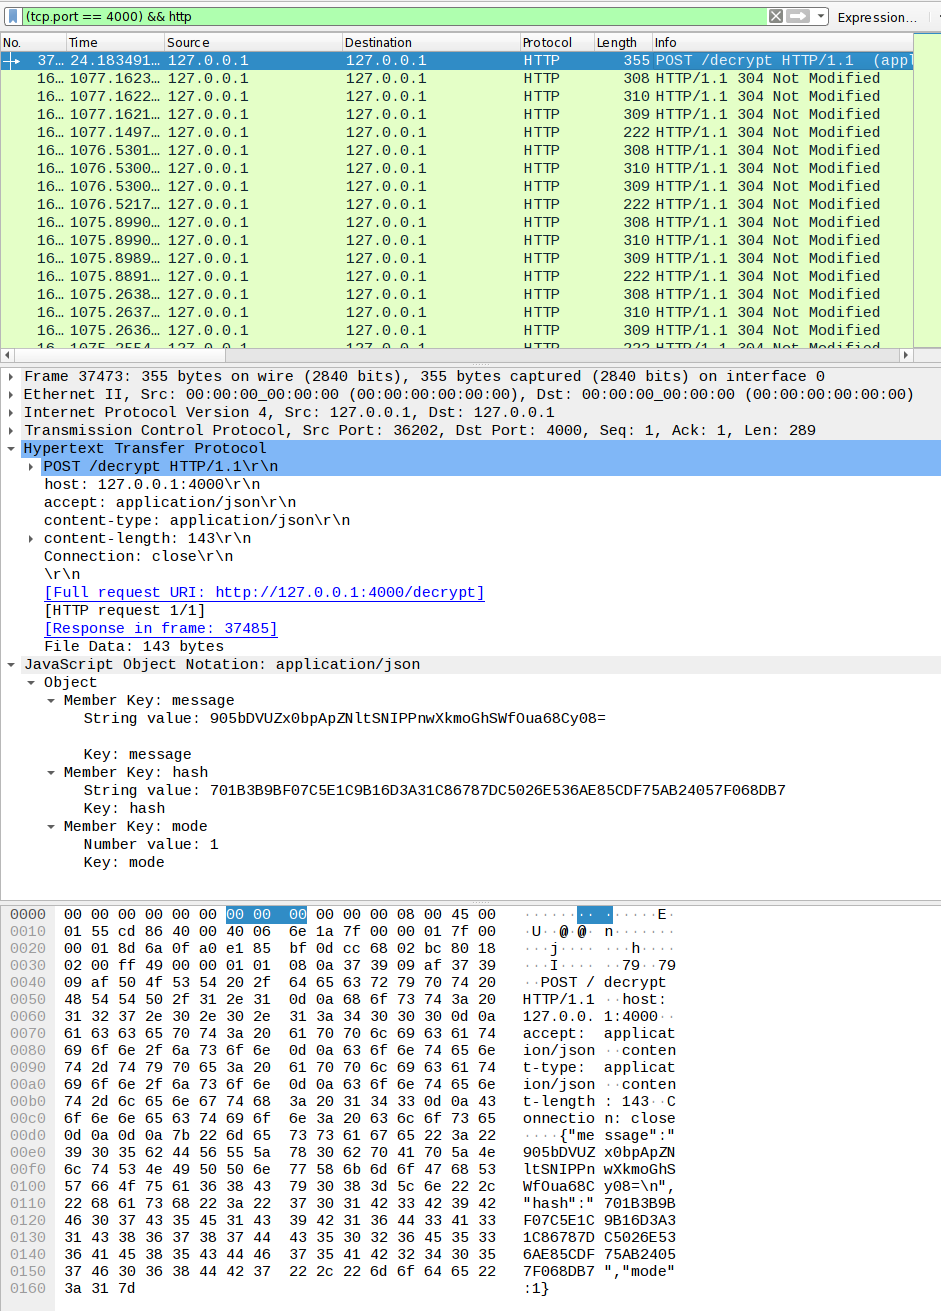
\includegraphics[width=1\textwidth]{Figures/b16.png}
  \caption[Node App at port 3000 sends ciphertext to Node App at port 4000 ]{Node App at port 3000 sends ciphertext to Node App at port 4000 }
  \label{fig:b16}
\end{figure}
\FloatBarrier


\begin{figure}[!h]
  \centering
      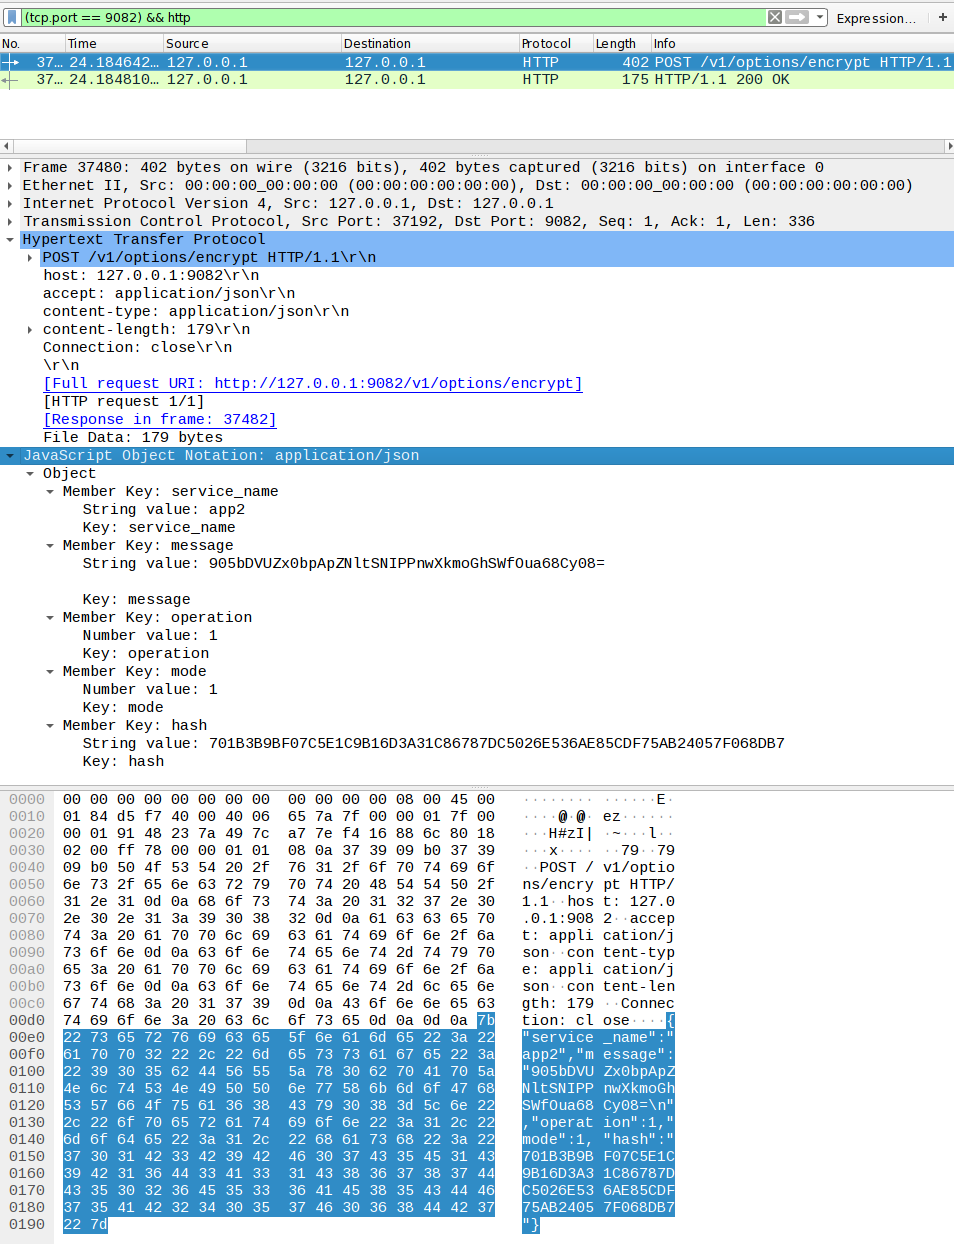
\includegraphics[width=1\textwidth]{Figures/b14.png}
  \caption[Node sends decryption message to the API ]{Node sends decryption message to the API }
  \label{fig:b14}
\end{figure}
\FloatBarrier

Now the node app on port 4000 needs to decrypt the ciphertext so it sends over its service name, ciphertext, operation is 1 this time for decryption, mode is 1 again and finally the hash of the plaintext forwarded from the other API to the API it is using on port 9082. This can all be seen in figure \ref{fig:b14}


\begin{figure}[!h]
  \centering
      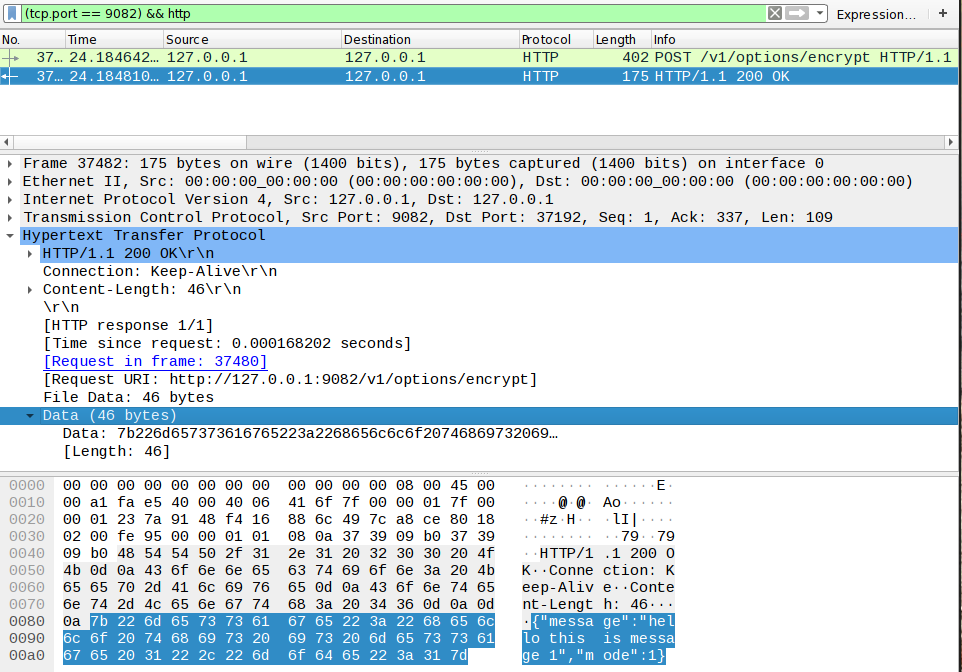
\includegraphics[width=1\textwidth]{Figures/b15.png}
  \caption[API responds with plaintext]{API responds with plaintext}
  \label{fig:b15}
\end{figure}
\FloatBarrier

Figure \ref{fig:b15} is a response from the API, the message was decrypted successfully and is simply sent back to the node app in plaintext the mode is also attached but this is not required for anything other than statistics. 


Next I would like to demonstrate the difference between the encryption modes using the node apps. Basically the point here is that if sending the same message i.e the same plaintext over and over in a non dynamic encryption environment the cipher text that will be produced will always be the same. 
You can see the following demonstration in video form which I mentioned before at this link https://www.youtube.com/watch?v=LsR4XsGrDCY&t=70s

Therefore since this project is all about dynamic encryption the ciphertext will be different every time if using the same plaintext. Note that it is guaranteed to be different every time if mode 2 is used since that will use a unique key for each message, mode 1 on the other hand is built for speed and therefore will use the latest available key therefore if frequent identical plaintexts are sent then there is a possibility that some of the ciphertexts will be the same. 

To test this properly a human would be too slow to type out the message each time so once again I will use a script which will basically submit the form on the browsers behalf. This python script is called send message.py and is once again located inside the GitHub repository.
The script looks like this.
\begin{lstlisting}
#!/usr/bin/env python3.7

import requests
import time

Service_address = "127.0.0.1"
Service_port = 3000

message = "hello -> using mode 1"
encrypt_mode = 1	# 1 for fast. i.e. encrypt using the latest key. 2 for secure only use 1 key once.

how_many_times = 10

url1 = "http://" + Service_address + ":" + str(Service_port) + "/encrypt"
data = {'message':message, 'encrypt_mode': encrypt_mode}

for i in range(0,how_many_times,1):
	print("sending")
	 
	r = requests.post(url = url1, data = data) 
	time.sleep(0.6)
\end{lstlisting}
As you can see this will send the message "hello -> using mode 1" to the encrypt route of the node app on port 3000 ( yes both the node app and the API have an encrypt route, only realised this might be confusing just now ).
This message will be sent 10 times and after each message is sent there will be a break for 0.6 seconds.
Firstly I will use encrypt mode 1.


\begin{figure}[!h]
  \centering
      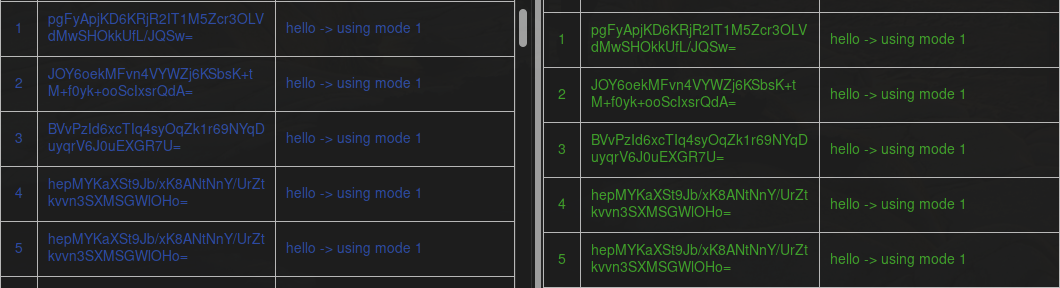
\includegraphics[width=1\textwidth]{Figures/b17.png}
  \caption[Encryption / Decryption mode 1 part 1]{Encryption / Decryption mode 1 part 1}
  \label{fig:b17}
\end{figure}
\FloatBarrier

\begin{figure}[!h]
  \centering
      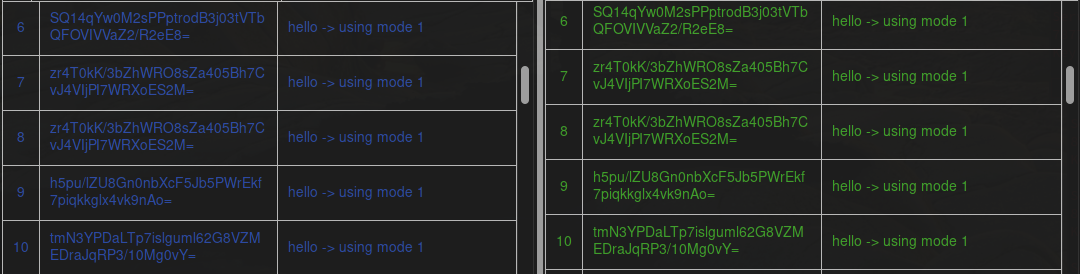
\includegraphics[width=1\textwidth]{Figures/b18.png}
  \caption[Encryption / Decryption mode 1 part 2]{Encryption / Decryption mode 1 part 2}
  \label{fig:b18}
\end{figure}
\FloatBarrier

Figures \ref{fig:b17} and \ref{fig:b18} show the output of the encryption and decryption table in the NodeJs apps after running the script. Here the plaintext is all the same and as you can see on the right node app they have decrypted successfully. The purpose of this test is to examine the cipher text and see which ones if any used the same key.
message 1 used a key unique to itself.
message 2 used a key unique to itself.
message 3 used a key unique to itself.

however message 4 and 5 have the same ciphertext therefore they have used the same key this is because by the time message 5 was encrypted no need key was generated yet and since this is mode 1 it just used the latest key available which happened to be the same one as message 4.

message 6 used a key unique to itself.

message 7 and 8 once again used the same key as each other.

message 9 used a key unique to itself.

message 10 used a key unique to itself.

Given that only two plaintexts were encrypted using the same key twice this is actually a very good result for mode 1. In my previous testing normally you would see three messages in a row encrypted with the same key. This time the keys were generated quicker than expected. How keys are generated will be covered in the sync-server section after this API section. 

Now we will have a look at using mode 2 for encryption to use mode 2 I simply modified two variables in the script.
\begin{lstlisting}
message = "hello -> using mode 2"
encrypt_mode = 2
\end{lstlisting}

\begin{figure}[!h]
  \centering
      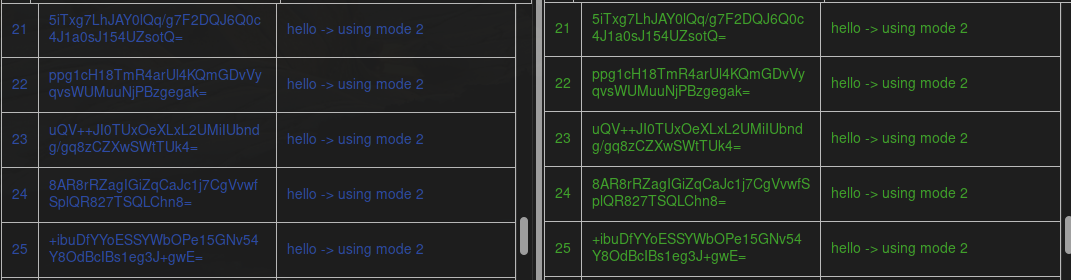
\includegraphics[width=1\textwidth]{Figures/b19.png}
  \caption[Encryption / Decryption mode 2 part 1]{Encryption / Decryption mode 2 part 1}
  \label{fig:b19}
\end{figure}
\FloatBarrier

\begin{figure}[!h]
  \centering
      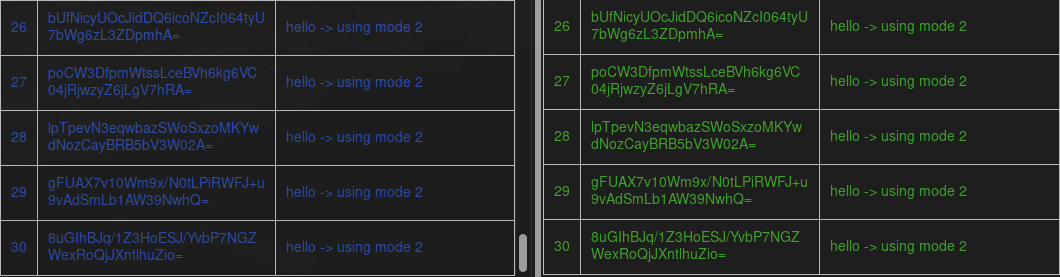
\includegraphics[width=1\textwidth]{Figures/b20.png}
  \caption[Encryption / Decryption mode 2 part 2]{Encryption / Decryption mode 2 part 2}
  \label{fig:b20}
\end{figure}
\FloatBarrier
Figures \ref{fig:b19} and \ref{fig:b20} show the output of the encryption and decryption table in the NodeJs apps after running the script with the modifications.
By looking at the ciphertexts part of the table of the Apps you can see that they are all different despite the same plaintext being used, therefore each message was encrypted using its own unique key and decrypted successfully as can be seen on the right app. 

This means that my algorithm works perfectly for both modes of operation.

As we can see both modes demonstrated dynamic cryptography. Mode 2 is in my opinion is more secure as each message no matter what is encrypted using a unique key. However there is a possibility that you will run out of suitable keys if sending loads of data frequently. If this happens you will just have to wait a little bit for new keys to be generated and encrypt again. 
Mode 1 therefore is perfect if you would like to send loads of data at regular intervals since there will be no issue with running out of keys, you will still reap the benefits of dynamic encryption since it takes around one second or so to generate new keys ( testing time of key generation will be seen later ). 

This will conclude the explanation and testing of aspects related to the API. If I were to explain everything related to the API it would take another 50 pages or so to go through everything therefore I selected the most impact full aspects of the API based on the outcomes of the project and left out most of the technical aspects. This section should have provided a good understanding of most of the more important operations of the API, it is recommended to browse through the GitHub repository for a full exposure of the API.  % Conclusions and Term 2 work
\chapter{Discussion and Conclusions}
\label{chap:conclusions}
\lhead{\emph{Discussion and Conclusions}}
%In this chapter, you should expand upon (and initially reflect upon) the discussion and conclusion of the research phase of the project. The expectation here is that you should discuss the results presented in the previous evaluation section of the project in their totality (i.e. as a whole) from which you will then draw clear conclusions both on the quantitative and qualitative aspects of the overall project. This chapter should be a about 2000 words long (5 pages of text - 1600 words of discussion and 400 words of conclusion). This may vary depending on quality. The conclusion section of this report should conclude the project.
%
%Some suggested sections (the nature of this chapter should be discussed in detail with your term 2 supervisor):
%
\section{Solution Review}
%Discuss how well your solution solves the problem, based on your results from the evaluation chapter.
The solution developed turned out to be successful and works well for an alpha version of the product. There are a number of improvements that still need to be made to use the system to its full potential. There are also a number of security features that need to be incorporated in order to prevent spoofing and denial of service attacks against peers, which will be discussed in the future work section.  

The solution successfully demonstrates the use of dynamic cryptography in a full fledged system containing the API, peer to peer network and the NodeJs App that uses said API in a simple messaging type of application. There are a number of encryption methods available that are dynamic in nature which was not planned initially however when coding the project it just seemed right to include different ways of using dynamic cryptography for various needs of the user. Currently DynamiCrypt supports two modes of dynamic encrypt, both were tested and work as expected.

The solution also demonstrates that by using tree parity machines it is possible to avoid public key crypto systems such as RSA. The design of DynamiCrypt also ensures that the keys never leave the process therefore the clients using the API have no idea what so ever about the keys or anything to do with the key store. The client only witnesses data going into the API and returning as cipher text and sending ciphertext to the API in return for the plaintext.

The solution turned out to be very performance orientated and performed faster that I have originally expected when it comes to generating keys. Originally I stated that it was acceptable for it to take around two seconds to generate a key however the current solution manages to generate a key in roughly one second.


\section{Project Review}
%Discuss how well you addressed the project, and what you might do differently if you were to do it again. Make sure to identify how you handled any problems that arose during the project. Identify key skills that you learnt during the project, and clearly describe how you applied these, and how you might apply them differently if you were to do a similar project.
The solution resulted in a completely different technique as originally described in semester one. This was more my fault as I believed the synchronisation could be done through the API alone and no other networking aspect was required. Fortunately after spending a lot of time learning how Boost Asio works I was able to create a peer to peer network capable of achieving the synchronisation task at a much quicker rate than it would be possible by simply using the Pistache framework. This was unexpected and for a few weeks I felt like I was behind as I was learning how to use Boost Asio however this slight setback didn't cause the project to fail. 

Overall I feel like I addressed the project quite well in the time frame available. I managed to create a functional API, a peer to peer network that is capable of handling multiple tree parity machines and a functional NodeJs app that uses the API in order to send encrypted messages between other NodeJs apps.

Initially I wanted to use the Cpprestsdk library to build the API as it was the most popular as well as being actively developed by Microsoft. This did not come to fruition due to the sample examples not compiling on my system after installing and linking the library during compilation. In order to solve this problem I began looking for alternative REST frameworks and stumbled upon Pistache which turned out to be more responsive than Cpprestsdk and even native PHP. This means that each request is processed in less time and more requests can be processed per second, which will reduce the time needed to synchronise the tree parity machines. Due to Pistache claiming to be written in pure C++11 with no external dependencies I was able to successfully compile the examples provided on their GitHub. 

Although Pistache is a great API library which I would definitely use for APIs I will build in the future, I believe this project would benefit in performance if the peers could integrate better with the API. Currently since the peer class is using Boost Asio I need to use global objects to interface with the API which is not ideal.

If I were to redo the project again, I would use Boost Asio for all of my networking needs as the API would be able to interface with the sync-server much more efficiently without the need of global objects. This will be implemented later on in a future version of DynamiCrypt but it would be handy to have done it from the start.

Another aspect of the project I would do differently if starting again is to change the way NodeJS apps register with the API. Currently is takes two API requests and multiple NodeJs to NodeJs requests before being able to begin synchronisation. This would take a while to plan out the way it should be done and perhaps a completely different method of doing it could be used.

A challenging part of this project was implementing the networking aspects of the solution using C++. I have used C++ in the past for small utility like programs that are normally complete in one or two days. I never used C++ for networking since using NodeJs or python is normally easier. DynamiCrypt is by far the largest and most complicated software I built single handily. Since C++ is object orientated it is easy to spread out the functionality and different aspects of the system into its own classes thereby I was able to easily manage and maintain this project. 

The API aspect of the project was fairly straight forward and I never ran into any issues with Pistache, this is because it is very similar to how you would structure a NodeJS rest API but of course the way you would parse JSON is very different. JavaScript handles its objects pretty much in JSON format whereas with C++ you can either do it manually by parsing strings or use a library like RapidJSON which is what I used. 

The peer class uses Boost ASIO network library which is very powerful and you can use it to build pretty much any type of network for your software. The library uses familiar patterns like callbacks and promises however it is implemented differently than what I'm used to in NodeJS and due to the wide nature of the library it took almost a month to learn how to use it effectively and produce the peer to peer network capabilities. I am glad that I did this since I am now familiar with one of the most popular and powerful networking C++ libraries. I choose to use C++ and stand by my choice as it is very fast primarily since it is a compiled language and is able to process networking traffic efficiently. Since DynamiCrypt is network heavy due to synchronisation it is able to process requests faster than NodeJs which was my second choice for this project and thus synchronise faster.        




\section{Future Work}
%Discuss any proposals for completion of the project, or for enhancements, or for re-design of your solution or software. Enumerate all the things you would have wanted to do should you have more time to work on this project.
DynamiCrypt is currently in early alpha stage, there are a large number of features and improvements that need to be made before I would be comfortable with people using DynamiCrypt as a real solution rather than a proof of concept. This section could go on for ever as software in general could continue to be constantly improved whether it is when someone finds a bug or some library you are using that receives an update and features being constantly requested by users, sections of any software can also be redesigned to become more efficient. 

Therefore for this section the most important aspects of DynamiCrypt will be listed, which will be implemented in the next milestone which I plan to work on in my spare time after college.

\begin{enumerate}
	\item (Tree parity machine structure, query based synchronisation) Structure of the tree parity machines would need to be slightly tweaked and simplified. Currently the neurons, weights and input vector are stored in a custom dynamic array type of data structure, to improve performance this should be replaced with something more light weight than a class and the structure would need to be updated anyway for the introduction of query based synchronisation. Currently DynamiCrypt's tree parity machines synchronise based on a random input vector as I didn't have time to implement the ideal method. With query based synchronisation tree parity machines will synchronise much faster since the queries are based on the weights of the tree parity machines rather than simply a random vector. Using queries will also improve security since the tree parity machines will synchronise much faster than the attacker could learn using his own tree parity machines. This would be the first improvement made as the time to generate the key should decrease by a reasonable amount, currently it takes around one second to generate a key on average by using queries this should decrease by 20-30 percent as demonstrated by other research papers in this topic.
	\item ( Peer data exchange ) Ideally when exchanging data between peers there should be confidentiality, integrity and authentication, and non-repudiation. Currently the peers just send raw TCP packets and trust that the peer that they are sending the data to is actually the peer they mean to communicate with. Provided that the attacker doesn't use any active attacks such as man in the middle attacks and sending custom built packets to the peers, otherwise the system currently is secure since the information sent over the network contains nothing relating to the key being generated so by purely listening to packets it would be unlikely to generate the key. In order to secure this from attacks such as man in the middle the peers would have to use some sort of MAC to provide integrity and authentication, and use digital signatures to provide non-repudiation.
	\item ( API ) At the moment the API server and the peers are using different networking libraries while running in the same process. Currently this works ok however later on when more features and complex interactions between the API and the peers is introduced this might cause some issues. Ideally the API server should have been written using Boost Asio library however due to time constraints and the fact that using Pistache library for the API was a lot quicker since it is a much more higher level library it was chosen for the alpha version of DynamiCrypt. Therefore the API would need to be rebuilt from scratch using the Boost Asio library and will then integrate seamlessly with the peers thereby getting rid of some of the global objects that are currently used to communicate between the API and the peer.
	The API would also need to have authentication implemented that way another localhost client would not be able to high jack the tree parity machines of the appropriate client.
	\item ( Modes of encryption ) Currently DynamiCrypt supports two modes of encryption. I have planned to implement two more. Mode 3 will be able to use the same key n number of times, this is sort of in between mode 1 and mode 2 where mode 1 can potentially use the same key as many times as it wants and mode 2 the key is only ever used once. Mode 4 will be like an ultra secure mode where the message will be split into n chunks and each piece will be encrypted with a different key.
	\item ( Multiple Tree parity machines per peer ) When synchronising a peer has one tree parity machine for each peer it is connected to. A more steady key income would occur if each peer was able to use lets say five tree parity machines per peer. An attempt was made to implement this feature and the code does handle multiple tree parity machines per peer the only issue is I was able to correctly setup the buffers and the data in the socket kept on becoming corrupted, in order to make sure the project was usable by the end of the semester I decided to implement this feature properly at a later date. 
	\item ( Random generator) To initialise the random weights of tree parity machines and create the random input vector the random function is seeded with the input from /dev/urandom this works well however for a serious cryptographic system it is better to use a more sophisticated method which I have yet to figure out.
\end{enumerate}
	There are many more things that would be implemented at a later stage however the above would be the initial changes I would make for the next version of DynamiCrypt.
	
\section{Conclusion}
%Enumerate the main conclusions you have got in terms of background, problem description and the solution approach you have come up with. Detail your primary and any secondary conclusions from your project.
The background aspect of this project was heavily tied to the solution because there was a number of ways dynamic encryption could be achieved. I discussed my initial methods in the later paragraph of this section and why I choose not to pursue them. This lead to a rather late start in the documentation of the background sections as I needed to make sure this was exactly how I aim to achieve this. Because dynamic encryption is rather uncommon and I just choose to do this because I have an interest in cryptography and security, there is no blogs, posts, videos or anything apart from research papers on my topic or in particular tree parity machines and synchronisation between them. However the research papers I uncovered did contain valuable information, formulas and implementation techniques which will suffice for building DynamiCrypt.

%problem description
The problem this project attempts to solve has been clear from the very beginning. I knew that I wanted to work on an encryption system that was capable of changing keys throughout the session between connected hosts without obviously sending the keys through the network. DynamiCrypt aims to provide an alternative method to standard public key cryptography methods like RSA. The dynamic encryption aspect of the project provides extra security so that even if the attacker managed somehow to steal the key, potentially only a small piece of the session could be accessible to the attacker and that small piece in relation to the whole session would be meaningless and any sensitive information should be safe.

%solution approach
The way I intended to achieve dynamic encryption varied a number of times. Initially I had difficulty in coming up with a reasonable way to achieve this. The difficulty originated due to the fact that the key should not be sent to the other host directly or at least in an obvious manner. Before finding out about the existence of tree parity machines I was going to base my encryption method to the one used by Dencrypt where the encrypted packets are layered with an unknown encryption method, this would mean that I would need to research many encryption methods and some way to detect or at least have the other host identify which encryption method was used. How Dencrypt achieved dynamic encryption was secret and they only provided a brief overview. I had no idea how to safely detect the encryption method without brute forcing every possible cipher which would be useless to begin with as an attacker would be able to do the same. My next idea was to have the initial host generate a large number of keys within which the real key would be held and have the host intelligently select and test potential keys using some sort of a trained AI algorithm, my reasoning behind this would be that the attacker would need to test each key which would take too long whereas the host with the AI engine would only need to test a relatively small number. However for this to be feasible the encryption technique must be relatively slow reducing the number of keys tested per second to a feasible minimum. And the file sent over to the other host with the keys would need to be tens of GigaBytes large and only contain one correct key, therefore making this idea useless. I needed some sort of way that allowed for the same data to be present on both hosts without specifically sending this data, magic I believed before stumbling upon synchronising tree parity machines. I found the idea of two neural networks learning from each other that eventually leads to them having the same weights fascinating. I knew then that this is how I will accomplish my project. 

Developing DynamiCrypt was the most enjoyable aspect of the project as you get to see a piece of software that you envisioned slowly but surely come to life. There were a few bumps and hiccups along the way that slowed down progress or discarded features in favour of getting the system to work by the end of the semester. However I am happy with what I have achieved and the fact that DynamiCrypt is functional and synchronises faster than I have anticipated. I would say the software is in alpha stage with many more refinements to come in the next version. 

\section{Code and Demo}
The code is available at the following GitHub link.
\begin{lstlisting}
https://github.com/ArtiomSu/DynamiCrypt
\end{lstlisting}
The demo is available on YouTube at the following link.
\begin{lstlisting}
https://www.youtube.com/watch?v=LsR4XsGrDCY
\end{lstlisting}



















































 % Conclusions and Term 2 work
\else
\chapter{Conclusions and Future Work}
\label{chap:conclusions}
\lhead{\emph{Conclusions}}
%This chapter should comprise 2-3 pages and enumerate conclusions of this phase of work. In your final report Discussions and Conclusions will form separate chapters and be significantly longer and more detailed.

\section{Discussion}
%A reflective discussion of some of the problems you encountered during this phase of the project and how that may influence how you proceed with the next phase.
This project uses a number of different libraries for different tasks. One of the most important tasks is getting the REST API to function properly. Initially I wanted to use the Cpprestsdk library as it was the most popular as well as being actively developed by Microsoft. This did not come to fruition due to the sample examples not compiling on my system after installing and linking the library during compiling. In order to solve this problem I began looking for alternative REST frameworks and stumbled upon Pistache which turned out to be more responsive than Cpprestsdk and even native PHP. This means that each request is processed in less time and more requests can be processed per second, which will reduce the time needed to synchronise the tree parity machines. Due to Pistache claiming to be written in pure C++11 with no external dependencies I was able to successfully compile the examples provided on their GitHub. 

Another problem that surfaced was due to my lack of knowledge about advanced C++ concepts while writing the prototype. I needed to use a generic data type, specifically the DynamicArray class needed to contain a generic variable and it needed a template function. I refreshed my knowledge on templates by watching a small number of tutorials such as this \cite{CppTotorial}. However I still had issues with linking during compilation. While trying to fix the issue I discovered \cite{cppHeaderCrap} that it is best to put function templates only in header files separating templates into header and definitions causes issues therefore The whole DynamicArray class now resides in a header file and has no corresponding .cpp file. I will have to reinforce my knowledge in other aspects of C++ as different challenges will arise throughout the project later on.

\section{Conclusion}
%Enumerate the main conclusions you have got in terms of background, problem description and the solution approach you have come up with.
The background aspect of this project was heavily tied to the solution because there was a number of ways dynamic encryption could be achieved. I discussed my initial methods in the third paragraph of this section and why I choose not to pursue them. This lead to a rather late start in the documentation of the background sections as I needed to make sure this was exactly how I aim to achieve this. Because dynamic encryption is rather uncommon and I just choose to do this because I have an interest in cryptography and security, there is no blogs, posts, videos or anything apart from research papers on my topic or in particular tree parity machines and synchronisation between them. However the research papers I uncovered did contain valuable information, formulas and implementation techniques which will suffice for building a proper tree parity machine. 


%problem description
The problem this project attempts to solve has been clear from the very beginning. I knew that I wanted to work on an encryption system that was capable of changing keys throughout the session between connected hosts without obviously sending the keys through the network. My current solution sends information through the network that helps build these keys however by grabbing this information and attempting to construct the key from it in theory is impossible. My project aims to improve security over just using standard methods, It can be argued that standard encryption methods are generally good enough and this is true it is very difficult to the point of almost impossible to decrypt data without the key that was been encrypted using standard encryption. However my project aims to go the extra mile that even if the attacker managed somehow to steal the key, potentially only a small piece of the session could potentially be accessible to the attacker and that small piece in relation to the whole session would be meaningless and any sensitive information should be safe.

%solution approach
The way I intended to achieve dynamic encryption varied a number of times. Initially I had difficulty in coming up with a reasonable way to achieve this. The difficulty originated due to the fact that the key should not be sent to the other host directly or at least in an obvious manner. Before finding out about the existence of tree parity machines I was going to base my encryption method to the one used by Dencrypt where the encrypted packets are layered with an unknown encryption method, this would mean that i would need to research many encryption methods and some way to detect or at least have the other host detect which encryption method was used since how Dencrypt achieved dynamic encryption was secret and they only provided a brief overview. I had no idea how to safely detect the encryption method without brute forcing every possible method which would be useless to begin with as an attacker would be able to do the same. My next idea was to have the initial host generate a large number of keys within which the real key would be held and have the host intelligently select and test potential keys using some sort of a trained AI algorithm, my reasoning behind this would be that the attacker would need to test each key which would take too long whereas the host with the AI engine would only need to test a relatively small number. However for this to be feasible the encryption technique must be relatively slow reducing the number of keys tested per second to a feasible minimum. And the file sent over to the other host with the keys would need to be tens of GigaBytes large and only contain one correct key, therefore making this idea useless. I needed some sort of way that allowed for the same data to be present on both hosts without specifically sending this data, magic I believed before stumbling upon synchronising tree parity machines. I found the idea of two neural networks learning from each other that eventually leads to them having the same weights fascinating. I knew then that this is how I will accomplish my project. On top of the tree parity machines I would need to have some sort of network interface that would allow the "syncing data" to travel to other hosts. And to make the dynamic encryption more dynamic there will be multiple tree parity machines synchronising which I believe would lead to a steady supply of secret keys. The diagrams provided earlier in this paper would suffice for achieving this system although I do fear that due to the many packets needed to synchronise a single tree parity machine never mind multiple will put a strain on the application which can be solved by running multiple instances which might surface issues regarding that, this however will be something to deal with in semester two.


\section{Future Work}
%Enumerate all the things you would have wanted to do should you have more time to work on this report.
Given the limited time available for actual code in semester one due to research among other things being the focus, the prototype ended up being very basic. There was no time to do anything worth showing using Pistache the REST framework. Ideally a simple server could have been setup with the desired routes and basic functionality that allows data to be bounced between two instances of the server. This could mimic the queries sent back and forward between the tree parity machines, since those queries are going to be sent using TCP or more specifically HTTPS this would give me a good start for next semester as it would be easy to replace meaningless data with query data.
The prototype uses random data for Tree Parity Machine input as it was quicker and easier to implement however ideally queries should have been used for security purposes and will definitely make an appearance in the final solution.

%Additional resources on the use of latex is below.

%Tutorials:
%\begin{itemize}
%    \item \url{https://www.latex-tutorial.com/tutorials/beginners/how-to-use-latex}
%    \item \url{https://en.wikibooks.org/wiki/LaTeX}
%    \item \url{https://www.sharelatex.com/learn/Main_Page}
%    \item \url{http://www.math.harvard.edu/texman}
%    \item \url{https://web.stevens.edu/hfslwiki/images/a/a0/ShareLatex_Tutorial.pdf}
%\end{itemize}

%Presentations:
%\begin{itemize}
%    \item \url{http://www.iu.hio.no/~frodes/rm/ppt/latex.ppt}
%    \item \url{https://classes.soe.ucsc.edu/ams200/Fall09/Latex_intro.ppt}
%    \item \url{http://www.menet.umn.edu/~blake/latexcourse/courseslides.ppt}
%\end{itemize}
 % Conclusions and Term 2 work
\fi


%% ----------------------------------------------------------------
\label{Bibliography}
\bibliographystyle{IEEEtranN}  % Use the "IEEE Transaction" BibTeX style for formatting the Bibliography
\bibliography{Bibliography}  % The references (bibliography) information are stored in the file named "Bibliography.bib"
\lhead{\emph{Bibliography}}  % Change the left side page header to "Bibliography"

%% ----------------------------------------------------------------
% Now begin the Appendices, including them as separate files

\addtocontents{toc}{\vspace{2em}} % Add a gap in the Contents, for aesthetics

\appendix % Cue to tell LaTeX that the following 'chapters' are Appendices

\chapter{Code Snippets}

%Put appendix material in this section e.g. code snippets 

%USE THE APPENDICES	% Appendix Title

%\chapter{Wireframe Models} % Appendix Title

%\input{Appendices/AppendixC} % Appendix Title

\addtocontents{toc}{\vspace{2em}}  % Add a gap in the Contents, for aesthetics
\backmatter
\end{document}  % The End
%% ----------------------------------------------------------------